% FCSG-Net B.Tech research project report.
% Built on the NIT Rourkela DissertationGuidelinesV4_5 template (copy kept in
% college_reference/). Needs the college bundle files listed in thesis/README.md
% (NITR.cls, FrontPages.tex, Ref/*.bst) before it will compile.
\documentclass[12pt,a4paper,oneside]{NITR}

\usepackage[hyphens]{url}
\usepackage[none]{hyphenat}
\usepackage{amsmath,amsfonts,mathdots,amssymb}  % template also loads yfonts (blackletter), unused here
\usepackage{graphicx}
\usepackage{xcolor}
\usepackage{tikz}
\usetikzlibrary{trees,shapes}
\usepackage{booktabs}
\usepackage{multirow}
\usepackage{longtable}
\usepackage{subcaption}
\usepackage{siunitx}            % aligned decimals in result tables
\sisetup{group-separator={,},group-minimum-digits=4}

% Report figures are already generated as vector PDFs by
% evaluation/build_technical_report.py. Reference them in place, do not copy.
\graphicspath{{figures/}{../output/pdf/fcsg-report-assets/}{../results/diagnostics/}}

% Shared macros. Keep this file small.

% Writer notes. Every \todo prints in red so nothing ships half-written.
% Before final submission: grep -rn '\\todo' thesis/ must return nothing.
\newcommand{\todo}[1]{\textcolor{red}{\textbf{[TODO:} #1\textbf{]}}}
% Where a number came from. Renders nothing, exists for reviewers of the .tex.
\newcommand{\evidence}[1]{}

\newcommand{\fcsg}{FCSG-Net}
\newcommand{\dB}{\,dB}
\newcommand{\expert}[1]{$E_{#1\times#1}$}   % \expert{7} -> E_{7x7}


\onehalfspacing
\begin{document}
\sloppy
% ---------------------------------------------------------------- front matter
% ======================================================================
% Front-page fields. STAND-IN layout: when the college FrontPages.tex
% arrives, copy these values into its fields and replace this file.
% ======================================================================
\reportTitle{FCSG-Net: Frequency-Band Spatial Expert Routing\\for Lightweight Composite Image Restoration}
\docType{Project Report}
\degree{Bachelor of Technology}
\dept{Computer Science and Engineering}
% Ascending order of roll number.
\authors{Akshat Mittal (123CS0954)\\Risav Rathi (123CS0957)\\Ramnath Thakur (123CS0965)}
\authorsInline{Akshat Mittal (123CS0954), Risav Rathi (123CS0957) and Ramnath Thakur (123CS0965)}
\newcommand{\supname}{Dr.\ Shyampada Mukherjee}
\supervisorOne{\supname}
\submitDate{November 2026}

\ackText{%
We thank our supervisor, \supname, for guiding us through this project.

We thank the Department of Computer Science and Engineering, National
Institute of Technology Rourkela, for the chance to do this work. Kaggle
gave us free GPU time. Without it we could not have trained four models for
200,000 updates each.

We thank the DIV2K authors for making their dataset public. We also thank
Kai Zhang and colleagues for releasing the FFDNet code and pretrained
weights, which let us check our implementation against a published result.

Last, we thank our families and friends for their patience and support.
}

\abstractText{%
Old photographs usually carry several kinds of damage at once. Optical blur,
lost resolution, sensor or film noise and lossy JPEG compression each hit a
different part of the image spectrum. We ask whether a very small
restoration network can make use of that. Our network, FCSG-Net, splits the
degraded image into low, mid and high frequency bands with fixed, soft radial
masks in the Fourier domain. Three shared convolutional experts, with
$7\times7$, $5\times5$ and $3\times3$ kernels, process every band. A small
gate picks the two best experts for each band at every pixel. The model has
97,088 parameters and costs 9.39 GFLOPs for a $256\times256$ input. We first
verified the implementation and reproduced the published FFDNet result to
within 0.01\,dB. We then trained FCSG-Net, DnCNN and two FFDNet variants from
scratch on the same synthetic composite degradation of DIV2K images, with one
schedule and one evaluation protocol. On 100 validation images FCSG-Net
reaches 27.24\,dB PSNR. DnCNN reaches 27.83\,dB and blind FFDNet 28.19\,dB,
and FCSG-Net uses 82.6\% fewer parameters than DnCNN. The low FLOP count did
not make it fast. On a Tesla T4 GPU it is the slowest of the four. The
learned routing varies across the image and follows the noise level, with
within-image correlations up to 0.81. Overriding the gate's choices at
inference costs 0.37\,dB on average. Frequency-band routing gives a small
model behaviour we can inspect. Within this budget, it does not make the
model more accurate or faster than simple convolutional baselines.
}

\keywords{image restoration, frequency decomposition, mixture of experts,
spatial routing, lightweight networks}
            % college file: title, names, roll nos, guide(s)

\coverPage
\titlePage
\certificateOfExamination

\certificateOneSupervisor
%\certificateTwoSupervisors

%\dedication                    % add \dedicationText in FrontPages.tex to use
\declaration
\acknowledgment
\abstract

\tableofcontents
\cleardoublepage
\addcontentsline{toc}{chapter}{List of Figures}
\listoffigures
\cleardoublepage
\addcontentsline{toc}{chapter}{List of Tables}
\listoftables
\cleardoublepage
\chapter*{List of Abbreviations}
\addcontentsline{toc}{chapter}{List of Abbreviations}
\begin{tabular}{@{}ll@{}}
AMP    & Automatic Mixed Precision \\
AWGN   & Additive White Gaussian Noise \\
CNN    & Convolutional Neural Network \\
DIV2K  & DIVerse 2K resolution image dataset \\
FFT    & Fast Fourier Transform \\
FLOP   & Floating-Point Operation \\
GFLOP  & $10^9$ Floating-Point Operations \\
GPU    & Graphics Processing Unit \\
JPEG   & Joint Photographic Experts Group (compression) \\
LPIPS  & Learned Perceptual Image Patch Similarity \\
MAC    & Multiply-Accumulate Operation \\
MoE    & Mixture of Experts \\
MSE    & Mean Squared Error \\
PSNR   & Peak Signal-to-Noise Ratio \\
ReLU   & Rectified Linear Unit \\
RMSE   & Root Mean Squared Error \\
SE     & Squeeze-and-Excitation \\
SSIM   & Structural Similarity Index \\
\end{tabular}

\cleardoublepage

% ---------------------------------------------------------------- main matter
\pagenumbering{arabic}
\pagestyle{fancy}
\renewcommand{\chaptermark}[1]{\markboth{#1}{}}
\renewcommand{\sectionmark}[1]{\markright{\textbf{Chapter \thechapter}}}

\chapter{Introduction}\label{ch:intro}

\section{Motivation}\label{sec:motivation}

An old photograph is rarely damaged in just one way. Take a print shot
through a soft lens on grainy film, scanned at low resolution and saved as a
heavily compressed JPEG. It carries all four defects, and each one hits a
different part of the spectrum. Optical softening removes high spatial
frequencies. Resampling throws away detail above a resolution limit and adds
interpolation artefacts. Sensor and film noise spreads energy roughly evenly
across frequencies. In natural images the true signal is weakest at high
frequencies, so that is where noise dominates. JPEG quantises the mid and
high frequency coefficients of each $8\times8$ block, which leaves blocking
and ringing.

Most learned restoration networks treat this mixture as a single problem.
DnCNN \cite{zhang2017dncnn}, a deep convolutional network, sees the whole
degraded image and learns to undo every corruption in it without being told
which is which. Transformer restorers such as Restormer
\cite{zamir2022restormer} work very well, but they have tens of millions of
parameters. An archive, a library or a hobbyist with modest hardware cannot
run them.

We started from a simple idea. If each corruption sits in its own frequency
band, we could split the image into bands explicitly and let a small network
pick a filter for every band at every location. A large kernel suits smooth,
slowly varying structure. A small kernel responds to fine detail and to the
high-frequency part of the noise. A learned gate chooses between them pixel
by pixel. We call the result \fcsg{}, a frequency-conditioned, spatially
gated network. We hold it to a strict budget of fewer than five million
parameters and fewer than ten GFLOPs for a $256\times256$ input.

\section{Problem statement}\label{sec:problem}

Let $f \in [0,1]^{H\times W\times3}$ be a clean RGB image and let
\begin{equation}
	x = \mathcal{D}(f;\, \theta), \qquad
	\theta = (\sigma_\text{blur},\, s,\, \sigma_n,\, q)
	\label{eq:degradation}
\end{equation}
be a degraded observation. $\mathcal{D}$ applies Gaussian blur of width
$\sigma_\text{blur}$, bicubic down- and up-sampling by a factor $s$, additive
Gaussian noise with standard deviation $\sigma_n$ and JPEG compression at
quality $q$. We draw $\theta$ at random for every image and never give it to
the restoration model. The task is to learn a mapping $g_\phi$ whose output
$\hat f = g_\phi(x)$ is close to $f$ in PSNR, SSIM and LPIPS. The network
must also meet two hard limits:
\begin{itemize}
	\item fewer than $5\times10^{6}$ trainable parameters, and
	\item fewer than 10 reported GFLOPs for one forward pass on a
	$256\times256$ RGB input.
\end{itemize}

\section{Hypothesis and objectives}\label{sec:objectives}

We test one hypothesis. \emph{Apply a fixed radial frequency decomposition,
then route each band per pixel to the top two of several shared
convolutional experts with different kernel sizes. The learned routing will
change with image content and with the degradation, the trained network will
depend on it for output quality, and the whole model will stay inside the
budget.} We wrote this as a claim to check, not as a promise that the network
beats anything.

The work has four objectives.
\begin{enumerate}
	\item[\textbf{O1}] Build \fcsg{} and check that it behaves as designed.
	The checks cover exact band reconstruction, the parameter and FLOP
	limits, memory, gradient flow and overfitting a single image
	(Chapters~\ref{ch:method} and~\ref{ch:setup}).
	\item[\textbf{O2}] Get baselines we can trust. We reproduce a published
	FFDNet result and train DnCNN on a Gaussian task with a known outcome
	(Chapter~\ref{ch:setup}).
	\item[\textbf{O3}] Train \fcsg{}, DnCNN and two FFDNet variants under one
	matched composite degradation protocol. Compare quality, size, compute and
	measured latency (Chapter~\ref{ch:results}).
	\item[\textbf{O4}] Describe what the router learned. Where does it send
	each band, how does that relate to the sampled degradation, and how much
	does the trained model rely on it (Chapter~\ref{ch:routing})?
\end{enumerate}

\section{Contributions}\label{sec:contributions}

This report makes four concrete contributions.
\begin{itemize}
	\item A restoration network that routes frequency bands spatially, with
	97,088 parameters and 9.39 reported GFLOPs at $256\times256$. We also give
	the tests showing the code matches the equations.
	\item A matched comparison. We train DnCNN, blind FFDNet, oracle FFDNet and
	\fcsg{} from scratch on the same synthetic composite degradation, with the
	same schedule, the same number of updates and the same evaluation
	protocol.
	\item A routing analysis. We relate per-pixel expert weights to the
	recorded degradation parameters and measure what happens when we override
	the gate at inference.
	\item A plain account of how it turned out. \fcsg{} reaches 27.24\dB{},
	against 27.83\dB{} for DnCNN and 28.19\dB{} for blind FFDNet, with 5.7
	times fewer parameters than DnCNN. It is not faster on a GPU. Its low FLOP
	count did not become low latency.
\end{itemize}
We make no claim of state-of-the-art quality. Frequency decomposition and
expert routing both have a long history (Chapter~\ref{ch:literature}). We
test one specific combination of them under a tight budget.

\section{Organisation of the report}\label{sec:organisation}

Chapter~\ref{ch:literature} reviews restoration networks, frequency-domain
methods and mixture-of-experts routing, and places \fcsg{} among them.
Chapter~\ref{ch:method} describes the degradation model and then the network
one module at a time. Chapter~\ref{ch:setup} covers the data pipeline,
baselines, training and evaluation protocols, and the verification runs.
Chapter~\ref{ch:results} reports restoration quality and computational cost.
Chapter~\ref{ch:routing} looks at the learned routing.
Chapter~\ref{ch:conclusion} sums up the findings and their limits and lists
the experiments we would run next. Appendix~\ref{app:repro} records what
anyone needs to reproduce the work, and Appendix~\ref{app:per-image} lists
results for every image.

\thispagestyle{empty}\cleardoublepage

\chapter{Background and Related Work}\label{ch:literature}
% LENGTH: 7-10 pages.
% SOURCE: notes/related.md is already written in prose. Adapt it, do not
% rewrite from scratch. Plan.md section 4 has the reading list.
% RULE: published numbers from other papers come from different datasets and
% protocols. Quote them as context only, never inside our results tables.

\section{Image Restoration with CNNs}\label{sec:lit-cnn}
% DnCNN (residual learning) and FFDNet (noise-level map, pixel unshuffle).
% Mention NAFNet as the efficiency reference and Restormer/SwinIR as the
% heavy end. Keep these two short.
\todo{adapt from notes/related.md "Foundations"}

\section{Frequency-Domain Restoration}\label{sec:lit-freq}
% MWCNN (wavelet subbands), FFC, SFNet/FSNet (closest neighbour, spend the
% most words here), FFTformer. Spectral bias (Rahaman) for motivation.
% The positioning sentence must be precise: SFNet does learned local frequency
% selection; we use FIXED radial masks then learned spatial expert mixing.
\todo{adapt}

\section{Mixture of Experts and Gating}\label{sec:lit-moe}
% Shazeer sparse MoE, Switch Transformer routing stability, load balancing
% vs our entropy regulariser. SE networks for the fusion block.
% Be honest: we compute every expert, so we get sparse WEIGHTS, not sparse
% COMPUTE. Say it here so the examiner does not find it later.
\todo{adapt}

\section{Evaluation Metrics}\label{sec:lit-metrics}
% PSNR, SSIM, LPIPS: one paragraph each with the formula for PSNR and what
% LPIPS measures, and why it can disagree with PSNR.
\todo{write}

\section{Research Gap}\label{sec:gap}
% Comparison table: rows = methods, cols = frequency decomposition? learned
% routing? spatial routing? params. Keep the old proposal gap table OUT unless
% MWCNN/SFNet/FFTformer are added to it (plan.md section 0.1).
\begin{table}[htbp]
	\centering
	\caption{Positioning of \fcsg{} against closely related methods.}
	\label{tab:gap}
	\begin{tabular}{@{}lcccl@{}}
		\toprule
		Method & Freq.\ split & Learned routing & Spatial & Notes \\
		\midrule
		DnCNN \cite{zhang2017dncnn}     & -- & -- & -- & residual CNN \\
		FFDNet \cite{zhang2018ffdnet}   & -- & -- & -- & noise map input \\
		MWCNN \cite{liu2018mwcnn}       & wavelet & -- & -- & joint subbands \\
		SFNet \cite{cui2023sfnet}       & learned & \todo{check} & \todo{check} & closest prior \\
		Sparse MoE \cite{shazeer2017moe}& -- & yes & -- & token routing \\
		\fcsg{} (ours)                  & radial FFT & top-2 & per pixel & 97k params \\
		\bottomrule
	\end{tabular}
\end{table}

\thispagestyle{empty}\cleardoublepage

\chapter{Proposed Method: \fcsg}\label{ch:method}

This chapter describes the synthetic degradation used for training and
evaluation, and then the network itself, one module at a time. The notation
follows the implementation in \texttt{models/fcsg.py} and
\texttt{models/blocks.py}.

\section{Degradation Model}\label{sec:degradation}

Archival photographs are degraded in a rough physical order: the lens softens
the image, scanning or resizing loses resolution, the sensor or film adds
noise, and lossy storage compresses whatever is left. Our synthetic pipeline
applies the four operations in that order (Table~\ref{tab:degradation}).
\begin{table}[htbp]
	\centering
	\caption{Composite degradation pipeline. Parameters are sampled independently for every image.}
	\label{tab:degradation}
	\begin{tabular}{@{}lll@{}}
		\toprule
		Stage & Parameter & Distribution \\
		\midrule
		Gaussian blur        & $\sigma_\text{blur}$ & $\mathcal{U}(0.5,\, 2.0)$ pixels \\
		Down/up resampling   & scale $s$            & $\mathcal{U}(1.0,\, 2.0)$, bicubic both ways \\
		Additive noise       & $\sigma_n$           & $\mathcal{U}(5,\, 50)/255$, clipped to $[0,1]$ \\
		JPEG compression     & quality $q$          & integer, uniform on $\{30,\dots,95\}$, 4:4:4 \\
		\bottomrule
	\end{tabular}
\end{table}

Blur uses Pillow's Gaussian filter. Resampling shrinks the image by $s$ with
bicubic interpolation and enlarges it back to the original size, so input and
output always have the same dimensions. Noise is additive white Gaussian noise
in 8-bit units, clipped to the valid range. JPEG encoding uses Pillow with
chroma subsampling disabled. The image is quantised to 8 bits before the
Pillow blur and before JPEG encoding, as a real file would be.

Each sample carries its four sampled parameters alongside the degraded and
clean images. The network never sees them. They are recorded so that, after
training, we can ask whether the router responds to the degradation
(Chapter~\ref{ch:routing}). With noise between 5 and 50 grey levels and JPEG
quality as low as 30, the mean input PSNR on our validation set is
20.99\dB{}.

\section{Architecture Overview}\label{sec:arch}

Figure~\ref{fig:architecture} shows the data flow. The degraded image $x$ is
split into a low, a mid and a high frequency band, each of which is an
ordinary RGB image. Three shared experts with $7\times7$, $5\times5$ and
$3\times3$ kernels process every band. A spatial gate assigns, at each pixel
and for each band, a weight to every expert, keeping only the two largest.
The weighted expert outputs form one restored image per band:
\begin{equation}
	y_b(u,v) = \sum_{e\in\{7,5,3\}} w_{b,e}(u,v)\; E_e(x_b)(u,v),
	\qquad b\in\{L,M,H\}.
	\label{eq:mix}
\end{equation}
The three band outputs are concatenated into nine channels, reweighted by a
squeeze-and-excitation block, projected back to RGB and refined. The network
predicts a residual that is added to its input:
\begin{equation}
	\hat{f} = x + \mathrm{Refine}\big(\mathrm{SEFusion}([\,y_L, y_M, y_H\,])\big).
	\label{eq:out}
\end{equation}

\begin{figure}[htbp]
	\centering
	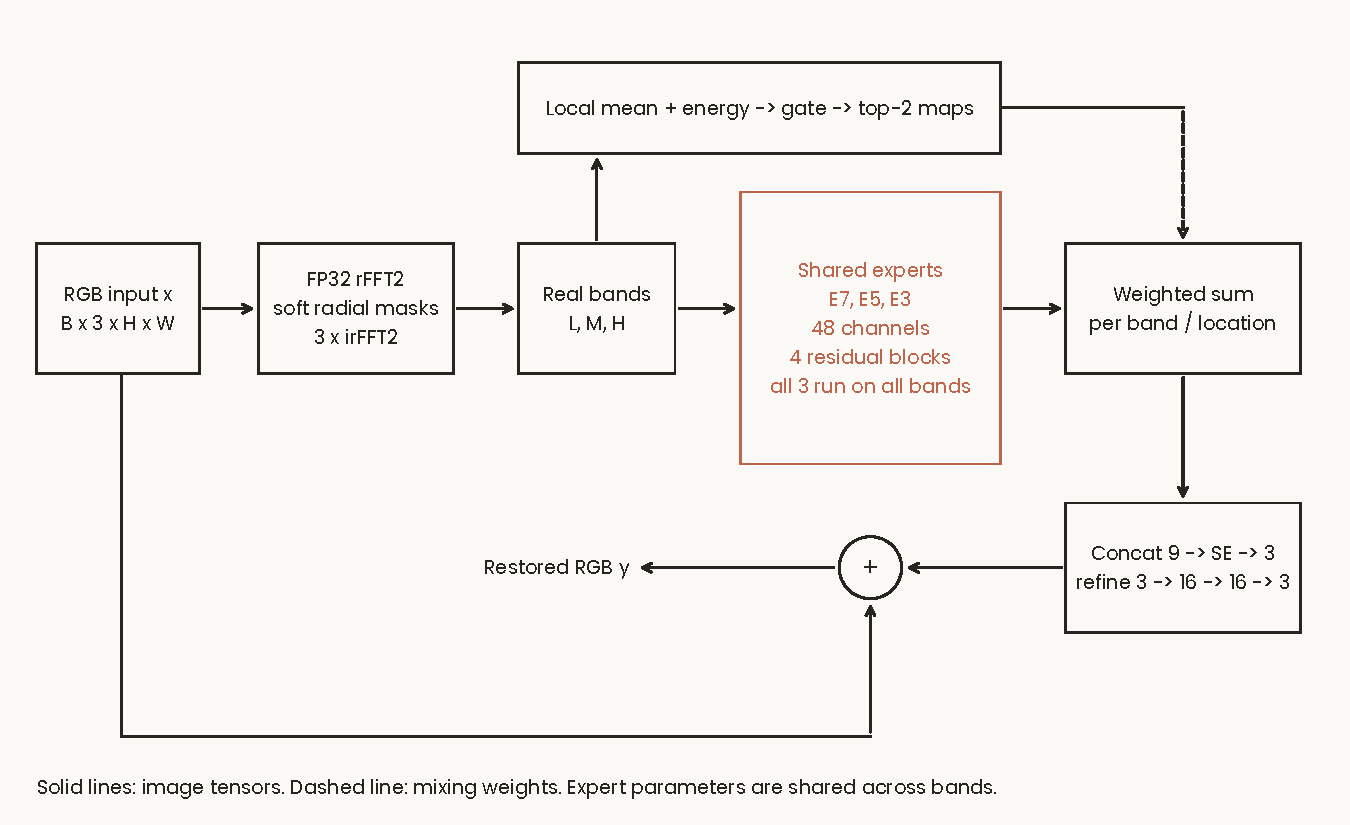
\includegraphics[width=\linewidth]{architecture.pdf}
	\caption{\fcsg{} data flow. Expert parameters are shared across the three
	bands; the band dimension is folded into the batch dimension before each
	expert call.}
	\label{fig:architecture}
\end{figure}

\section{Frequency Decomposition}\label{sec:freqdecomp}

The decomposition is done in the Fourier domain with fixed masks, but the
result of each mask is returned to the spatial domain immediately. We made
this choice early and deliberately. An earlier version of the proposal fed
masked complex spectra straight into the convolutional experts. That has two
problems. A convolution over a spectrum has no clean meaning, since
multiplication in one domain corresponds to convolution in the other, so the
argument that large kernels suit smooth structure no longer applies. And
complex inputs either become two real channels, where phase is discontinuous
and training becomes unstable, or require complex tensor support that many
PyTorch operations lack. Masking in frequency and filtering in space keeps
the decomposition exact and lets every expert be a plain real-valued CNN.

Let $X = \mathcal{F}(x)$ be the two-dimensional real FFT of the image with
orthonormal scaling, and let $r = \sqrt{f_x^2 + f_y^2}$ be the radial
frequency in cycles per pixel. Frequencies are built with \texttt{fftfreq}
and \texttt{rfftfreq} in the unshifted order the FFT uses. Each axis reaches
the Nyquist limit at $0.5$ cycles per pixel. A soft low-pass mask with cutoff
$c$ and transition width $\Delta = 0.05$ is a raised cosine:
\begin{equation}
	t_c(r) = \mathrm{clip}\!\left(\frac{r-c}{\Delta} + \tfrac12,\ 0,\ 1\right),
	\qquad
	\mathrm{LP}_c(r) = \tfrac12\big(1 + \cos(\pi\, t_c(r))\big).
	\label{eq:lowpass}
\end{equation}
With cutoffs $r_1 = 0.10$ and $r_2 = 0.25$, the three band masks are
\begin{equation}
	M_L = \mathrm{LP}_{r_1}, \qquad
	M_M = \mathrm{LP}_{r_2} - \mathrm{LP}_{r_1}, \qquad
	M_H = 1 - \mathrm{LP}_{r_2},
	\label{eq:masks}
\end{equation}
and each band image is $x_b = \mathcal{F}^{-1}(M_b \cdot X)$.

Three properties matter. First, the masks sum to one at every frequency, and
the FFT is linear, so $x_L + x_M + x_H = x$ exactly; no information is lost
or invented by the split. We measured a maximum reconstruction error of
$6.0\times10^{-7}$ in single precision. Second, the cutoffs are defined in
cycles per pixel rather than in FFT bin indices. A bin index means a
different physical frequency at $128\times128$ than at full resolution, so
bin-based cutoffs would shift between training crops and test images. With
normalised radii the same sinusoid falls in the same band at both sizes,
which we verified at 128 and 256 pixels. Third, the transitions are smooth.
A hard step in frequency produces ringing in space, and the network would
spend capacity undoing artefacts of its own preprocessing.

The FFT runs in single precision even during mixed-precision training,
because half-precision CUDA FFTs only support power-of-two sizes.
Figure~\ref{fig:masks} plots the three masks.

\begin{figure}[htbp]
	\centering
	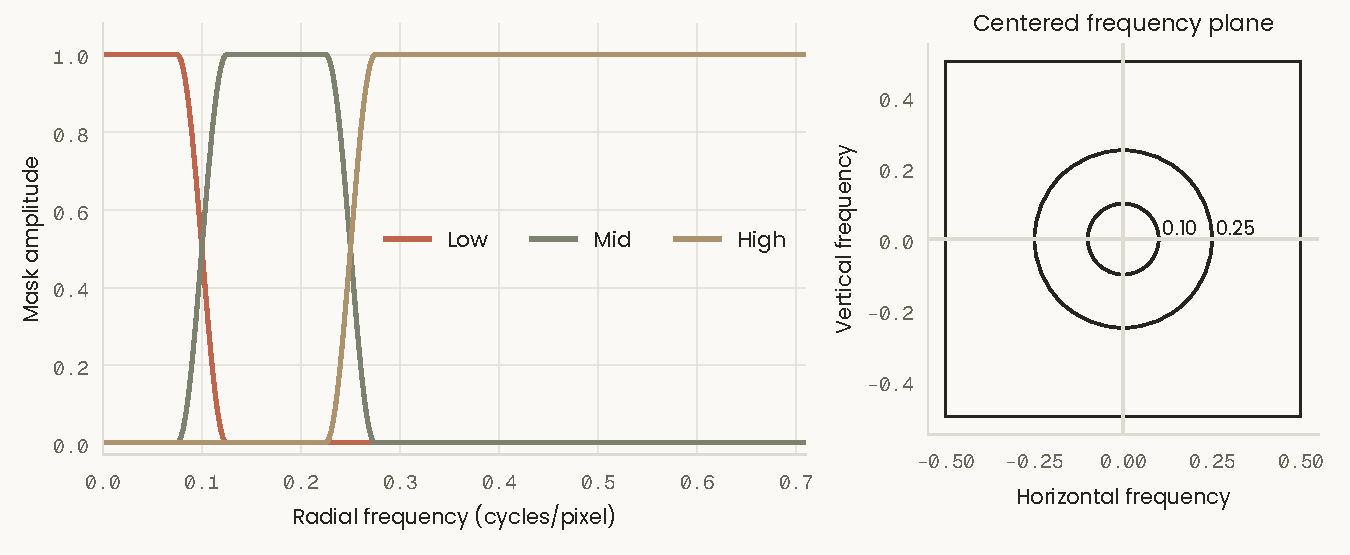
\includegraphics[width=0.9\linewidth]{frequency_masks.pdf}
	\caption{Raised-cosine band masks with cutoffs 0.10 and 0.25 cycles per
	pixel and transition width 0.05. Right: the masks on a centred frequency
	plane (the computation itself uses unshifted ordering).}
	\label{fig:masks}
\end{figure}

\section{Shared Kernel-Size Experts}\label{sec:experts}

There are three experts, $E_7$, $E_5$ and $E_3$, identical except for their
kernel size. Each one processes all three bands, so the parameters are shared
across bands and the number of experts does not grow with the number of
bands.

An expert first applies a lossless $2\times2$ pixel unshuffle
\cite{shi2016espcn}, turning a three-channel image into twelve channels at
half resolution, as FFDNet does. A $1\times1$ convolution expands these to 48
channels, followed by ReLU. Four residual blocks follow. Each block contains
two depthwise-separable stages \cite{chollet2017xception}: a $k\times k$
depthwise convolution and a $1\times1$ pointwise convolution, with a ReLU
after the first stage. A $1\times1$ tail maps back to twelve channels and is
added to the unshuffled input, and a pixel shuffle restores the original
resolution. Odd image sizes are padded by replication and cropped back.

Separable convolutions and half-resolution processing are what make the
budget possible. The experts run nine times per image, once per band for each
of three experts, and dense full-resolution convolutions at width 48 would
exceed ten GFLOPs by a wide margin.

We refer to the experts only by kernel size. Labels such as ``texture
expert'' or ``edge expert'' would be claims about what the experts learned,
and we have no attribution experiment that supports them.

\section{Spatial Top-2 Gate}\label{sec:gate}

A routing decision that is made once per image would amount to nine numbers
computed from a handful of global statistics. That is closer to a lookup
table than to a router, and it is likely to settle on a near-constant choice.
The \fcsg{} gate instead decides per location, so that a smooth sky and a
textured roof in the same photograph can be treated differently.

The gate stacks the three RGB bands into nine channels and computes, in
non-overlapping $16\times16$ windows, the local mean and the local mean of
squares of each channel. These eighteen statistics pass through a
two-layer $1\times1$ network ($18\to24\to9$, ReLU in between) that outputs
nine logits $a_{b,e}$, one per band and expert. The logits are divided by a
temperature $\tau = 1$ and bilinearly upsampled to full resolution. At each
pixel and for each band the two largest logits are kept and normalised with a
softmax; the third expert gets zero weight:
\begin{equation}
	w_{b,e}(u,v) =
	\begin{cases}
		\dfrac{\exp a_{b,e}(u,v)}{\sum_{j\in\mathcal{T}_b(u,v)} \exp a_{b,j}(u,v)}
		& e \in \mathcal{T}_b(u,v),\\[2ex]
		0 & \text{otherwise},
	\end{cases}
	\label{eq:topk}
\end{equation}
where $\mathcal{T}_b(u,v)$ is the set of the two highest-scoring experts.
The gate also returns the dense softmax over all three experts, $p_{b,e}$,
which is used by the entropy term of the loss. The whole gate has 681
parameters. Figure~\ref{fig:gate} shows the expert and gate operations.

\begin{figure}[htbp]
	\centering
	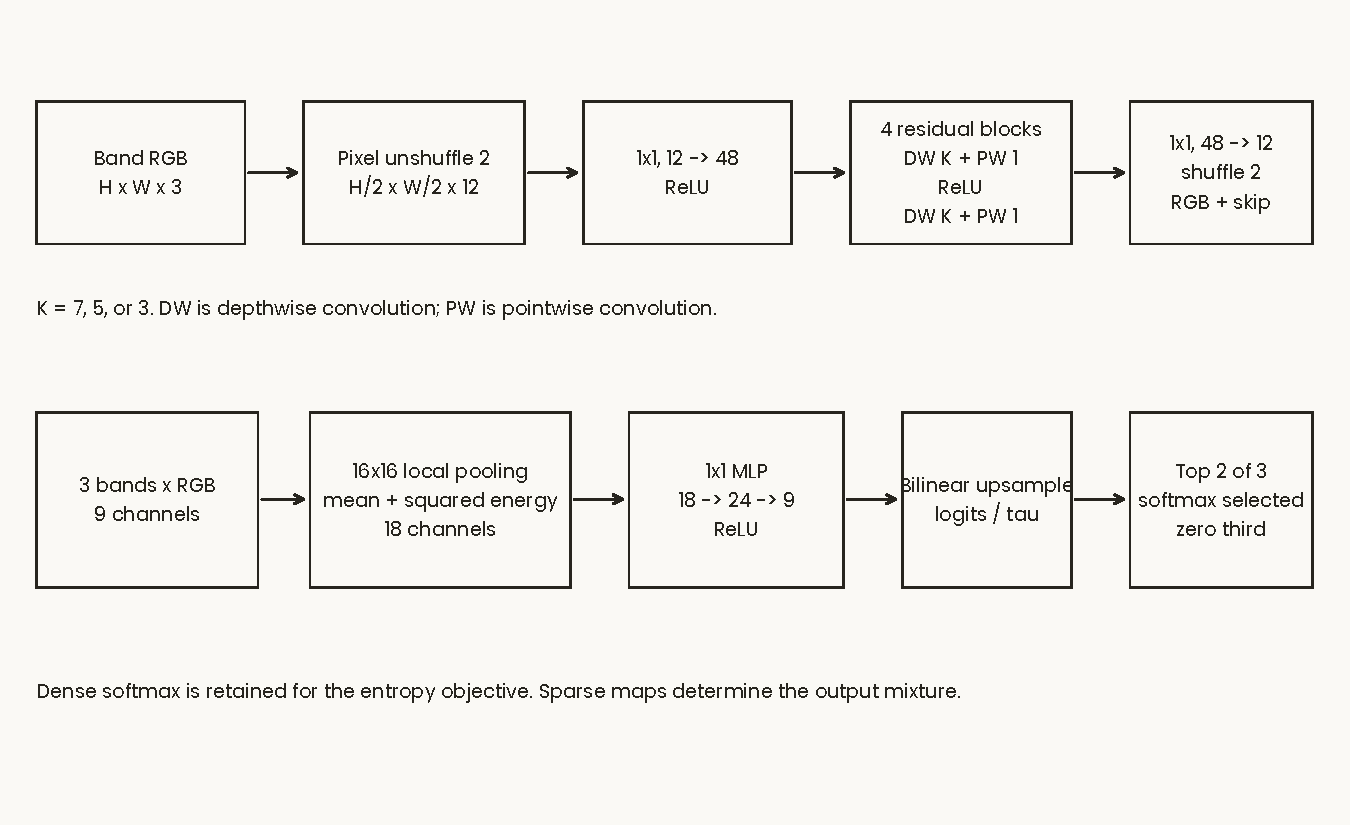
\includegraphics[width=0.9\linewidth]{expert_gate.pdf}
	\caption{Expert and gate operations. Experts use pixel rearrangement and
	depthwise-separable residual blocks; the gate pools band statistics in
	$16\times16$ windows.}
	\label{fig:gate}
\end{figure}

As noted in Section~\ref{sec:lit-moe}, every expert is evaluated before
mixing. Expert outputs at locations with zero weight are computed and then
multiplied by zero. Turning the sparse weights into saved computation would
require tiled conditional dispatch, which we did not implement.

\section{Fusion and Residual Refinement}\label{sec:fusion}

The three weighted band outputs are concatenated into nine channels. A
squeeze-and-excitation block \cite{hu2018se} pools them globally, passes them
through a $9\to3\to9$ bottleneck with a sigmoid, and scales each channel. A
$1\times1$ convolution projects the result to three channels. Three
$3\times3$ convolutions ($3\to16\to16\to3$, ReLU between them) refine it, and
the output is added to the degraded input as in Equation~\eqref{eq:out}.
Predicting a residual rather than the image itself is the central lesson of
DnCNN \cite{zhang2017dncnn}, and it lets the network start from the identity.

\section{Training Objective}\label{sec:loss}

The loss has three terms:
\begin{equation}
	\mathcal{L} = \mathcal{L}_\text{char}
	+ 0.05\,\mathcal{L}_\text{freq}
	+ \lambda_\text{ent}(t)\,\mathcal{L}_\text{ent}.
	\label{eq:loss}
\end{equation}

The Charbonnier loss \cite{charbonnier1994} is a smooth variant of L1,
\begin{equation}
	\mathcal{L}_\text{char} = \operatorname{mean}\sqrt{(\hat f - f)^2 + \varepsilon^2},
	\qquad \varepsilon = 10^{-3},
\end{equation}
which behaves like L2 near zero and like L1 for large errors.

The frequency term is the mean absolute value of the orthonormal FFT of the
prediction error, $\mathcal{L}_\text{freq} = \operatorname{mean}\lvert
\mathcal{F}(\hat f - f)\rvert$. It weights errors at every frequency equally,
which counteracts the tendency of pixel losses to favour the dominant low
frequencies.

The entropy term is the negative dense routing entropy, summed over bands and
averaged over the batch and pixels:
\begin{equation}
	\mathcal{L}_\text{ent} = \sum_b \operatorname{mean}_{n,u,v}\sum_e p_{b,e}\log p_{b,e}.
\end{equation}
Minimising it maximises entropy, which keeps all three experts in use early
in training so that none of them is starved of gradient. A constant entropy
bonus would, however, push the router towards uniform weights forever, which
is the opposite of what we want to observe. The coefficient therefore decays
linearly, $\lambda_\text{ent}(t) = 0.01\,(1 - t/T)$, reaching zero at the
last update $T$. Because the sign of this term is easy to flip by accident,
the verification suite checks that it decreases as the weights approach
uniform. DnCNN and FFDNet are trained with the same Charbonnier and
frequency terms and no entropy term.

\section{Model Size and Complexity}\label{sec:size}

Table~\ref{tab:params} breaks down the 97,088 parameters. Almost all of them
are in the three experts; the gate, fusion and refinement stages together
account for under four thousand.

\begin{table}[htbp]
	\centering
	\caption{\fcsg{} parameter breakdown.}
	\label{tab:params}
	\begin{tabular}{@{}lr@{}}
		\toprule
		Module & Parameters \\
		\midrule
		Shared $7\times7$ expert            & 39,228 \\
		Shared $5\times5$ expert            & 30,012 \\
		Shared $3\times3$ expert            & 23,868 \\
		Spatial gate ($18\to24\to9$)        & 681 \\
		SE fusion and $9\to3$ projection    & 96 \\
		Residual refinement                 & 3,203 \\
		\midrule
		Total                               & 97,088 \\
		\bottomrule
	\end{tabular}
\end{table}

For compute we profile multiply-accumulate operations (MACs) with
\texttt{thop}, count each MAC as two floating-point operations, and add an
estimate of $12 \times 5N\log_2 N$ for the forward and inverse FFTs, with
$N = 256^2$. Small elementwise operations are not counted. Under this
convention a $256\times256$ forward pass costs 4.66 GMACs, or 9.39 GFLOPs
including the FFT estimate, inside the 10 GFLOP limit. The same convention is
applied to the baselines. As Chapter~\ref{ch:results} shows, this count turned
out to be a poor predictor of actual running time.

\thispagestyle{empty}\cleardoublepage

\chapter{Experimental Setup and Verification}\label{ch:setup}

The numbers in Chapter~\ref{ch:results} are only as good as the code and
protocol behind them. This chapter describes the data, the baselines and how
every model was trained and evaluated, and then the tests we ran before
committing GPU time to long training runs.

\section{Dataset and Data Pipeline}\label{sec:data}

All experiments use DIV2K \cite{agustsson2017div2k}, which provides 800
high-resolution training images and 100 validation images. Training uses only
the training split; the 100 validation images are used for every result we
report. Because we did not hold out a separate test set, the reported numbers
are validation results, a limitation we return to in
Chapter~\ref{ch:conclusion}.

Our first data loader decoded a full-resolution PNG for every crop, and
training ran at roughly 1.8 steps per second because the GPU waited on the
CPU. We replaced it with a cache of 32 fixed $128\times128$ crops from each
training image, 25,600 tiles in all, stored as a single 1.26\,GB array of
8-bit pixels and memory-mapped at training time. Random flips and
90-degree rotations augment the cached crops. The degradation of
Section~\ref{sec:degradation} is still applied on the fly by four loader
workers, so every epoch sees freshly sampled blur, scale, noise and JPEG
settings. In effect the set of degraded pairs is unlimited, while the set of
clean crops is fixed (Figure~\ref{fig:pipeline}).

\begin{figure}[htbp]
	\centering
	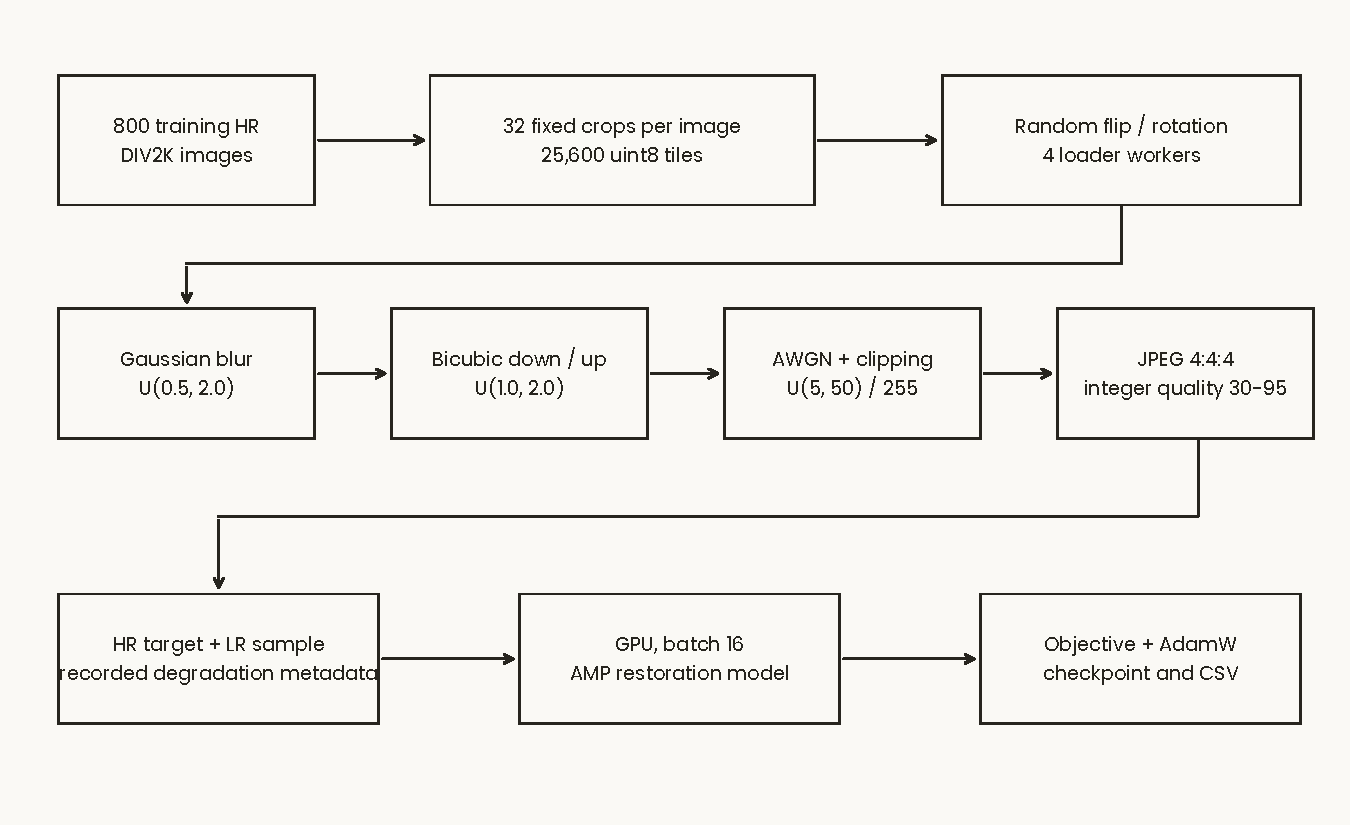
\includegraphics[width=\linewidth]{pipeline.pdf}
	\caption{Training data pipeline. Loader workers sample degradation
	parameters for each augmented clean crop and return the degraded input, the
	clean target and the parameters.}
	\label{fig:pipeline}
\end{figure}

Online degradation is good for training but awkward for anyone trying to
reproduce exact inputs. We therefore also exported a fixed set of 5,000
degraded and clean pairs generated with seed 1234, together with a manifest of
their parameters. The degradation code reproduces this set byte for byte, and
a single CPU worker generates about 233 samples per second.

\section{Baselines}\label{sec:baselines}

\paragraph{DnCNN.} Our RGB DnCNN has 17 convolutional layers of width 64
with batch normalisation and predicts the residual, giving 558,403
parameters.

\paragraph{FFDNet.} Our FFDNet follows the author's colour architecture
\cite{kair}: pixel unshuffle, 12 convolutional layers of width 96 and a
noise-level map concatenated to the input, giving 852,108 parameters. On our
composite task the noise map is a problem, because there is more to the
degradation than Gaussian noise. We therefore train two variants.
\emph{Oracle} FFDNet receives the true sampled noise level $\sigma_n$ as its
map. This is information no real user would have, so the oracle variant is an
upper reference rather than a fair competitor. \emph{Blind} FFDNet receives
a constant map of $27.5/255$, the middle of the noise range, during both
training and evaluation. It sees exactly what DnCNN and \fcsg{} see.

All four models are trained from scratch on the same composite degradation.
We do not compare against numbers published for other tasks or datasets.

\section{Training Protocol}\label{sec:training}

Every model is trained with the same configuration (Table~\ref{tab:hparams}),
differing only in the model and, for FFDNet, the noise map. The original plan
called for 300,000 updates; we reduced this to 200,000 to fit the weekly GPU
quota available to us.

\begin{table}[htbp]
	\centering
	\caption{Training configuration, identical for every method.}
	\label{tab:hparams}
	\small
	\begin{tabular}{@{}ll@{}}
		\toprule
		Setting & Value \\
		\midrule
		Optimiser            & AdamW \cite{loshchilov2019adamw}, weight decay 0 \\
		Learning rate        & $2\times10^{-4}$, cosine decay \cite{loshchilov2017sgdr} to $10^{-6}$ \\
		Updates              & 200,000 \\
		Batch                & 16 crops of $128\times128$ RGB \\
		Loss                 & $\mathcal{L}_\text{char} + 0.05\,\mathcal{L}_\text{freq}$, plus entropy term for \fcsg{} \\
		Entropy coefficient  & 0.01, linear decay to 0 (\fcsg{} only) \\
		Precision            & FP16 mixed precision \cite{micikevicius2018amp} with gradient scaling \\
		Validation           & 16 fixed crops every 2,000 updates \\
		Checkpoints          & every 2,000 updates (model, optimiser, scaler, step) \\
		Hardware             & NVIDIA Tesla T4 (Kaggle) \\
		\bottomrule
	\end{tabular}
\end{table}

Training ran in Kaggle notebook sessions, which stop after twelve hours.
Each run therefore resumes from its newest checkpoint at start-up. Checkpoints
store the model, optimiser, gradient scaler, step and configuration. They do
not store random number generator or sampler state, so a resumed run is not
bit-identical to an uninterrupted one. Training seeds were not fixed, and
each model was trained once. Recorded training-loop time was 10.06 hours for
\fcsg{}, 6.66 for DnCNN, 2.04 for blind FFDNet and 2.33 for oracle FFDNet.
Figure~\ref{fig:schedules} shows the learning-rate and entropy schedules.

\begin{figure}[htbp]
	\centering
	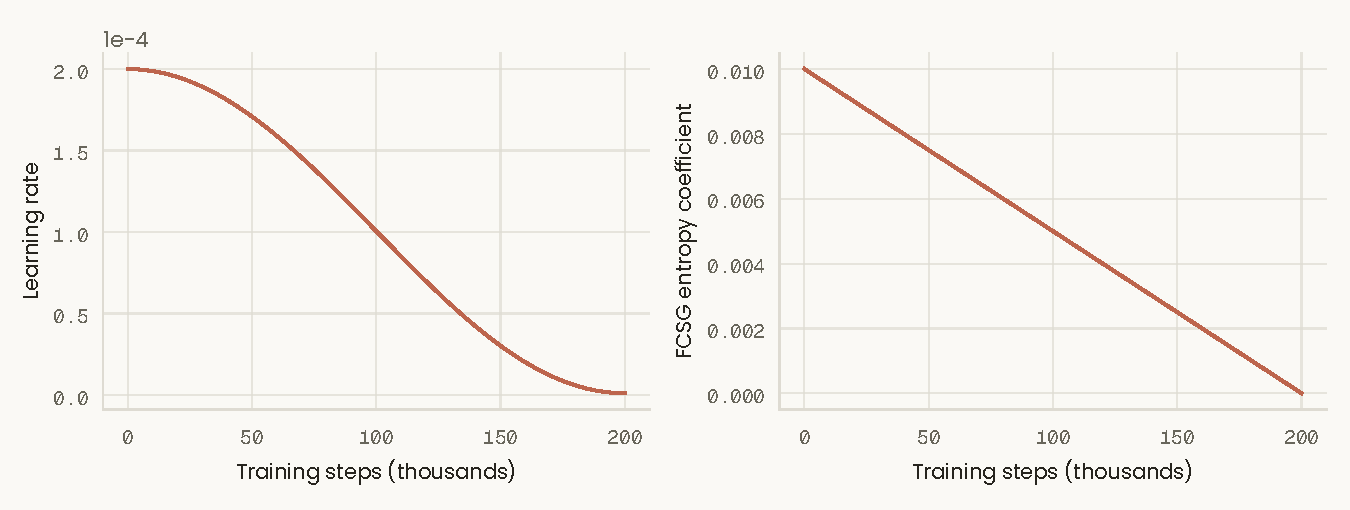
\includegraphics[width=0.85\linewidth]{schedules.pdf}
	\caption{Learning-rate and entropy-coefficient schedules over 200,000 updates.}
	\label{fig:schedules}
\end{figure}

\section{Evaluation Protocol}\label{sec:evalproto}

Final results use all 100 DIV2K validation images. Each image is degraded
once with a seed equal to its index, so every model sees exactly the same
degraded inputs. Inference is tiled: $256\times256$ tiles with 32 pixels of
overlap (stride 224), with the last tile in each direction aligned to the
image border and overlapping outputs averaged uniformly. Tiling keeps memory
low on large images; Section~\ref{sec:latency} measures how much it costs in
accuracy. Restored values are clipped to $[0,1]$ before computing PSNR, SSIM
and LPIPS as described in Section~\ref{sec:lit-metrics}.

During training we monitored a different quantity: PSNR on 16 fixed
$128\times128$ validation crops. The two are not comparable. For \fcsg{} the
final crop PSNR is 30.59\dB{} while the full-image result is 27.24\dB{}.
Crop numbers are used only for convergence curves.

\section{Implementation Verification}\label{sec:verification}

Before any long training run we ran a fixed set of checks in a single
notebook on the same Kaggle T4 (Python 3.12, PyTorch 2.10 \cite{paszke2019pytorch},
CUDA 12.8). The notebook stops at the first failure. Table~\ref{tab:gates}
lists the checks and their measured values.

\begin{table}[htbp]
	\centering
	\caption{Pre-training verification checks (Tesla T4, 25 September 2026 run).}
	\small
	\label{tab:gates}
	\begin{tabular}{@{}lll@{}}
		\toprule
		Check & Criterion & Measured \\
		\midrule
		FFDNet weights, CBSD68 $\sigma{=}25$ & within 0.5\dB{} of 31.21 & 31.220\dB \\
		Band reconstruction & $x_L{+}x_M{+}x_H = x$ & max error $6.0\times10^{-7}$ \\
		Frequency units & same band at 128 and 256 px & passed \\
		Parameter budget & $< 5$M & 97,088 \\
		Compute budget & $< 10$ GFLOPs at $256^2$ & 9.39 \\
		Memory, forward + backward & $< 4$ GB & 0.60 GB \\
		Shapes, gradients, odd sizes (AMP) & no errors & passed \\
		One-image overfit, 200 steps & MSE $<0.01$, $<\frac14$ initial & ratio 0.18 \\
		Checkpoint restore & identical outputs & passed \\
		Degradation reproducibility & byte-identical & passed \\
		\bottomrule
	\end{tabular}
\end{table}

Two of these checks deserve a word. The band reconstruction assertion is a
single line, yet it catches nearly every sign, shift and normalisation bug an
FFT implementation can have. The overfit test asks the full model to memorise
one image in 200 steps. A model that cannot do this has a bug, and finding
that out in a few seconds is far cheaper than finding it after ten hours of
training. \fcsg{} reduced the MSE from 0.0261 to 0.0046
(Figure~\ref{fig:overfit}). The memory figure was measured at batch size 1
and does not describe peak memory at the training batch size.

\begin{figure}[htbp]
	\centering
	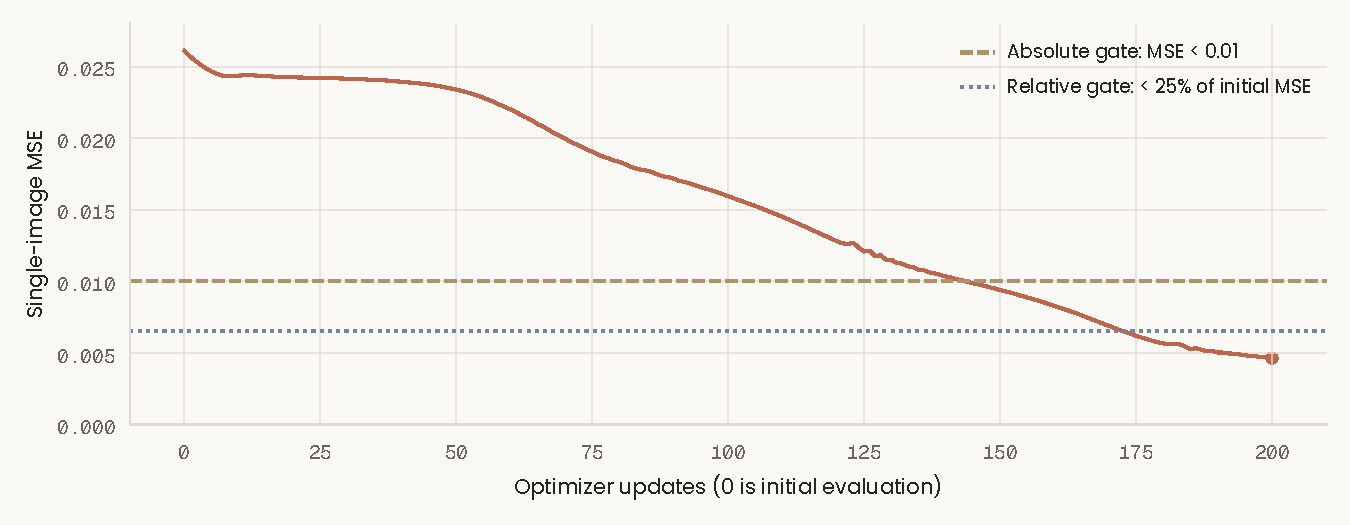
\includegraphics[width=0.75\linewidth]{overfit.pdf}
	\caption{Single-image overfit test: MSE over 200 updates.}
	\label{fig:overfit}
\end{figure}

\section{Baseline Reproduction}\label{sec:baseline-repro}

\paragraph{FFDNet.} To check our FFDNet implementation and evaluation code
against a published number, we loaded the author's pretrained colour weights
\cite{kair} and evaluated them on all 68 CBSD68 images
\cite{martin2001bsd} with unclipped Gaussian noise at $\sigma=25$, following
the author's protocol. We obtained 31.220\dB{}, against 31.21\dB{} in the
paper \cite{zhang2018ffdnet}, a difference of 0.01\dB{}. This verifies the
architecture, weight loading and evaluation path. It does not reproduce
FFDNet's training, which is why all composite models are trained from
scratch.

\paragraph{DnCNN.} As an end-to-end test of our training loop we trained
DnCNN on clipped Gaussian noise at $\sigma=25$ before moving to the composite
task. At checkpoint 286,000 it reached 32.65\dB{} on DIV2K validation and
31.04\dB{} on CBSD68 (Table~\ref{tab:gaussian}). These figures use clipped
noise and are not directly comparable with the unclipped protocol of the
FFDNet paper; they confirm that the training and evaluation code work on a
problem with a known order of magnitude.

\begin{table}[htbp]
	\centering
	\caption{DnCNN on clipped Gaussian noise, $\sigma=25$, checkpoint 286,000.}
	\label{tab:gaussian}
	\begin{tabular}{@{}lrrr@{}}
		\toprule
		Dataset & Images & Input PSNR & Output PSNR \\
		\midrule
		CBSD68           & 68  & 20.53\dB & 31.04\dB \\
		DIV2K validation & 100 & 20.70\dB & 32.65\dB \\
		\bottomrule
	\end{tabular}
\end{table}

\thispagestyle{empty}\cleardoublepage

\chapter{Restoration Results and Computational Cost}\label{ch:results}

This chapter reports how well the four trained models restore the 100 DIV2K
validation images, how their quality relates to size and compute, and what
they cost to run. Every model in this chapter was trained once, for 200,000
updates, under the protocol of Chapter~\ref{ch:setup}.

\section{Quantitative Comparison}\label{sec:main-table}

Table~\ref{tab:main} gives the main result. All models start from the same
degraded inputs, with a mean PSNR of 20.99\dB{}.

\begin{table}[htbp]
	\centering
	\caption{Composite restoration on 100 DIV2K validation images after 200,000
	updates. Gain is output minus input PSNR (input 20.992\dB{}). GFLOPs at
	$256\times256$.}
	\label{tab:main}
	\small
	\begin{tabular}{@{}lrrrrrr@{}}
		\toprule
		Method & PSNR$\uparrow$ & Gain & SSIM$\uparrow$ & LPIPS$\downarrow$ & Params & GFLOPs \\
		\midrule
		DnCNN                     & 27.831 & 6.838 & 0.7795 & 0.3242 & 558,403 & 73.43 \\
		FFDNet, blind             & 28.190 & 7.197 & 0.7899 & 0.3176 & 852,108 & 27.89 \\
		FFDNet, oracle$^\dagger$  & 28.240 & 7.247 & 0.7920 & 0.3162 & 852,108 & 27.89 \\
		\fcsg{}                   & 27.243 & 6.250 & 0.7529 & 0.3961 &  97,088 &  9.39 \\
		\bottomrule
		\multicolumn{7}{@{}l}{\footnotesize $^\dagger$Given the true sampled noise level; an upper reference, not a fair competitor.}
	\end{tabular}
\end{table}

\fcsg{} improves the input by 6.25\dB{}, which shows that the network learns
a substantial restoration, but it is the weakest of the four models on all
three metrics. It trails DnCNN by 0.59\dB{} and blind FFDNet by 0.95\dB{}.
The gap is larger in LPIPS than in PSNR: 0.396 against 0.318 for blind
FFDNet, which suggests that \fcsg{} leaves more visible residue than its PSNR
deficit alone would indicate.

The comparison looks different once size and compute are included
(Table~\ref{tab:tradeoff}). \fcsg{} reaches within 0.6\dB{} of DnCNN with
82.6\% fewer parameters and 87.2\% fewer reported FLOPs, and within 1\dB{}
of both FFDNet variants with 88.6\% fewer parameters and 66.3\% fewer FLOPs.

\begin{table}[htbp]
	\centering
	\caption{\fcsg{} relative to each baseline.}
	\label{tab:tradeoff}
	\begin{tabular}{@{}lrrr@{}}
		\toprule
		Compared with & PSNR difference & Fewer parameters & Fewer GFLOPs \\
		\midrule
		DnCNN           & $-0.588$\dB & 82.6\% & 87.2\% \\
		FFDNet, blind   & $-0.947$\dB & 88.6\% & 66.3\% \\
		FFDNet, oracle  & $-0.997$\dB & 88.6\% & 66.3\% \\
		\bottomrule
	\end{tabular}
\end{table}

Two observations about the baselines are worth recording. Blind FFDNet is the
strongest fair model, even though its noise map is a constant and so carries
no information. Its advantage over DnCNN therefore comes from the
architecture, most likely the half-resolution processing that gives each
layer a larger effective receptive field, rather than from noise
conditioning. Second, the oracle map adds only 0.05\dB{} over the blind
constant. Knowing the noise level helps little when blur, resampling and
JPEG artefacts are mixed in, because the map describes only one of the four
corruptions.

Figure~\ref{fig:benchmark} plots the three metrics side by side.

\begin{figure}[htbp]
	\centering
	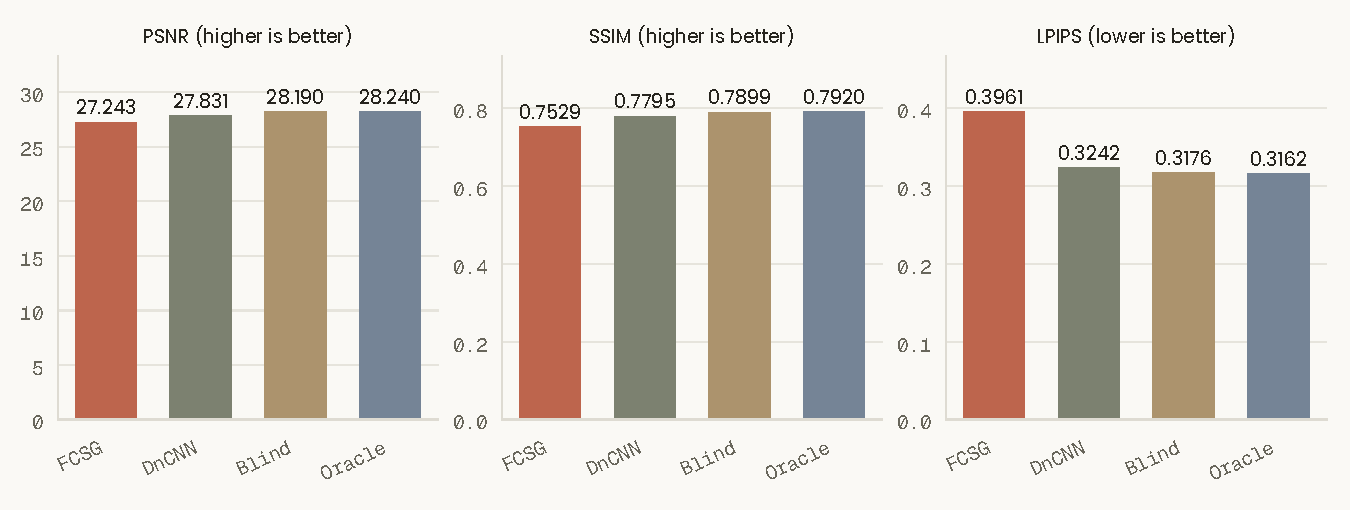
\includegraphics[width=\linewidth]{benchmark.pdf}
	\caption{Mean PSNR, SSIM and LPIPS over the 100 validation images. Each bar
	is one training run.}
	\label{fig:benchmark}
\end{figure}

Each model was trained once with an unfixed seed, so we cannot separate the
effect of the architecture from run-to-run variation. Differences of a few
hundredths of a decibel, such as the one between the two FFDNet variants,
should not be over-read. The gap between \fcsg{} and the baselines is large
enough, and consistent enough across images (Section~\ref{sec:per-image}),
that we do not expect a second seed to reverse it.

\section{Per-Image Analysis}\label{sec:per-image}

Averages can hide a model that wins on most images and loses badly on a few.
Table~\ref{tab:wins} compares \fcsg{} with each baseline image by image.

\begin{table}[htbp]
	\centering
	\caption{Per-image PSNR comparison of \fcsg{} against each baseline, 100 images.}
	\label{tab:wins}
	\begin{tabular}{@{}lccc@{}}
		\toprule
		Compared with & Wins / ties / losses & Mean difference & Range \\
		\midrule
		DnCNN          & 6 / 1 / 93  & $-0.59$\dB & $-2.75$ to $+2.07$\dB \\
		FFDNet, blind  & 0 / 0 / 100 & $-0.95$\dB & $-3.12$ to $-0.04$\dB \\
		FFDNet, oracle & 0 / 0 / 100 & $-1.00$\dB & $-3.48$ to $-0.07$\dB \\
		\bottomrule
	\end{tabular}
\end{table}

The deficit is systematic. Both FFDNet variants beat \fcsg{} on every one of
the 100 images. Against DnCNN, \fcsg{} wins on six images, and on one of them
by 2.07\dB{}, so the two convolutional designs fail in different places.
Image 0801 is an example: DnCNN barely improves it (28.09 to 28.22\dB{}),
while \fcsg{} reaches 29.32\dB{}. Conversely, DnCNN is the only model that
makes some images worse; three of its outputs score below their inputs.

The hardest image for every model is 0828, whose degraded input scores only
17.10\dB{}. \fcsg{} reaches 17.93\dB{} on it and the baselines between 18.61
and 18.83\dB{}. Our experiment does not isolate which of the four sampled
corruptions makes this image so difficult. Figure~\ref{fig:per-image} shows
the paired differences and the error distributions. The full table is in
Appendix~\ref{app:per-image}.

\begin{figure}[htbp]
	\centering
	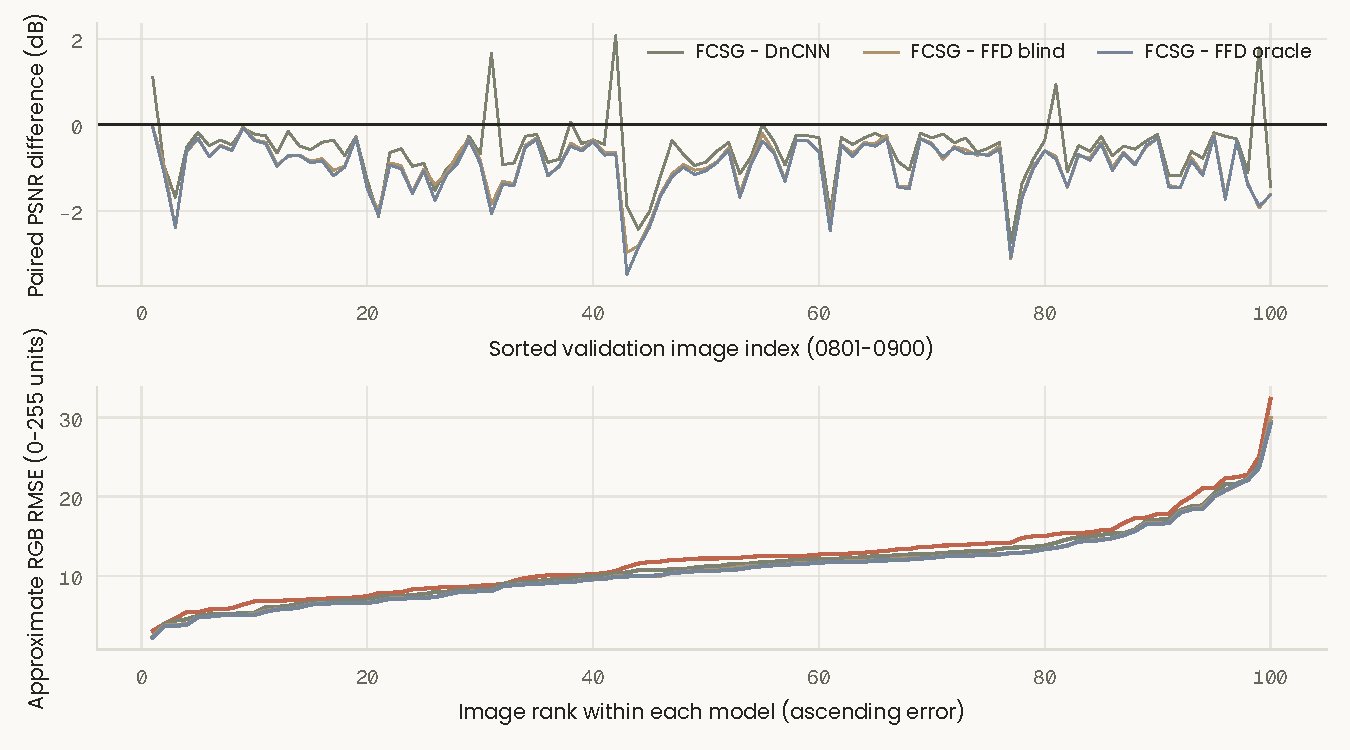
\includegraphics[width=\linewidth]{per_image_errors.pdf}
	\caption{Left: per-image PSNR difference between \fcsg{} and each baseline.
	Right: sorted per-image RMSE for every model (in 8-bit units).}
	\label{fig:per-image}
\end{figure}

\section{Qualitative Results}\label{sec:qualitative}

Figures~\ref{fig:qual-a} and~\ref{fig:qual-b} show the top-left
$320\times320$ region of validation images 0801 and 0802 for each model.
Every model receives the identical degraded input. PSNR labels refer to the
whole image, not the displayed region.

\begin{figure}[htbp]
	\centering
	\begin{subfigure}{\linewidth}
		\centering
		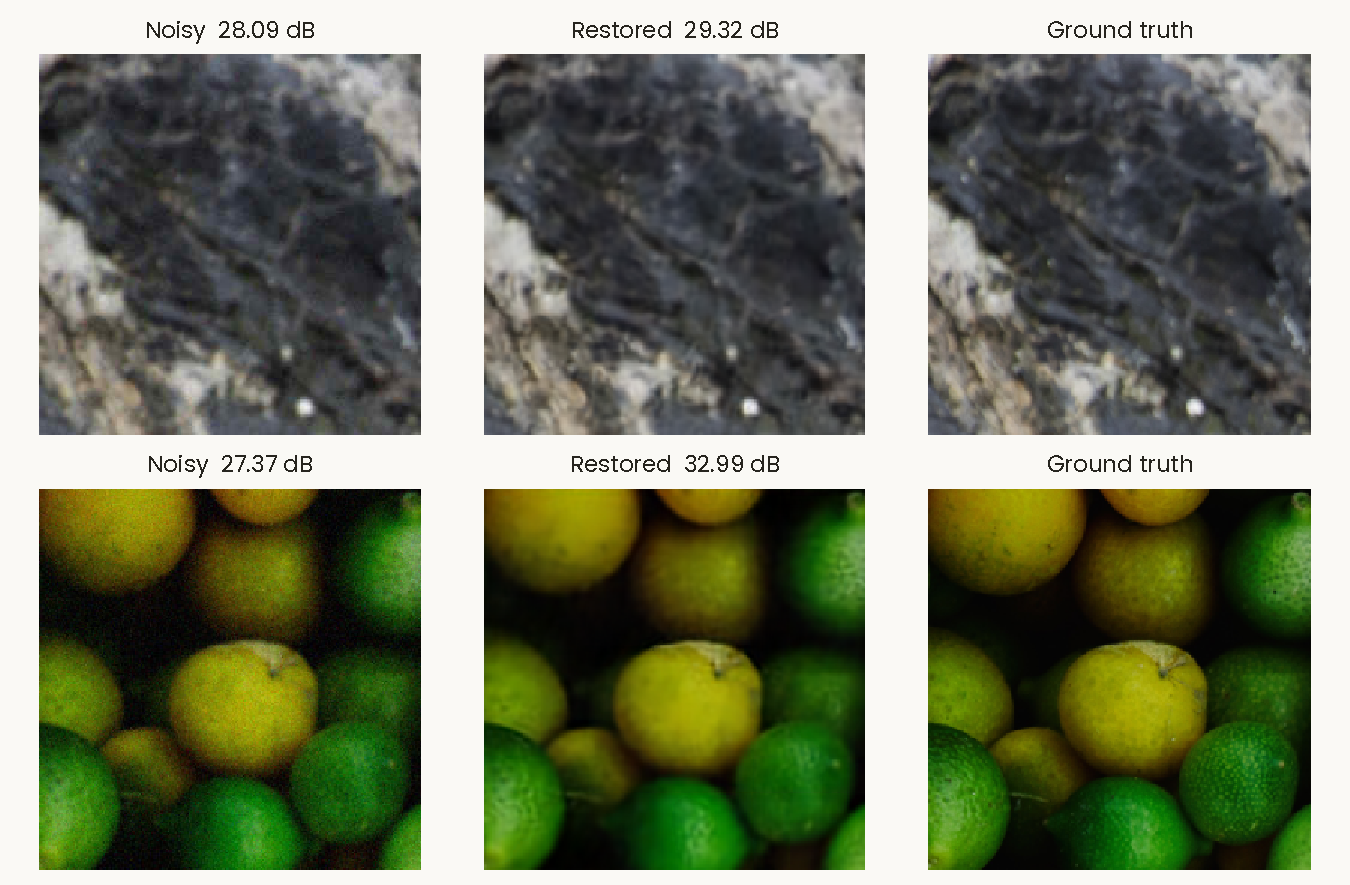
\includegraphics[width=0.92\linewidth]{qualitative_fcsg.pdf}
		\caption{\fcsg{}}
	\end{subfigure}\\[1ex]
	\begin{subfigure}{\linewidth}
		\centering
		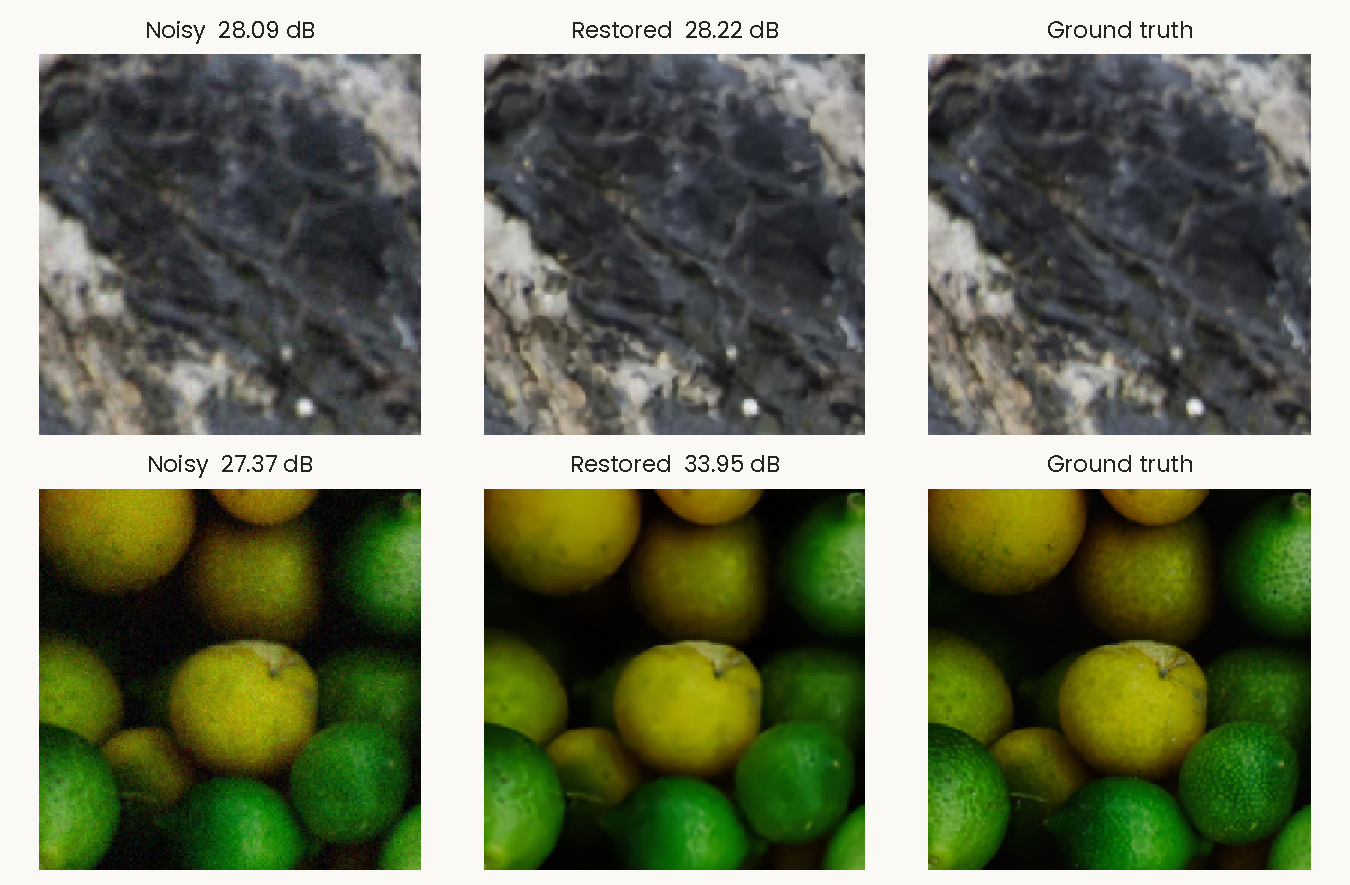
\includegraphics[width=0.92\linewidth]{qualitative_dncnn.pdf}
		\caption{DnCNN}
	\end{subfigure}
	\caption{Degraded input, restoration and clean target for \fcsg{} and DnCNN.}
	\label{fig:qual-a}
\end{figure}

\begin{figure}[htbp]
	\centering
	\begin{subfigure}{\linewidth}
		\centering
		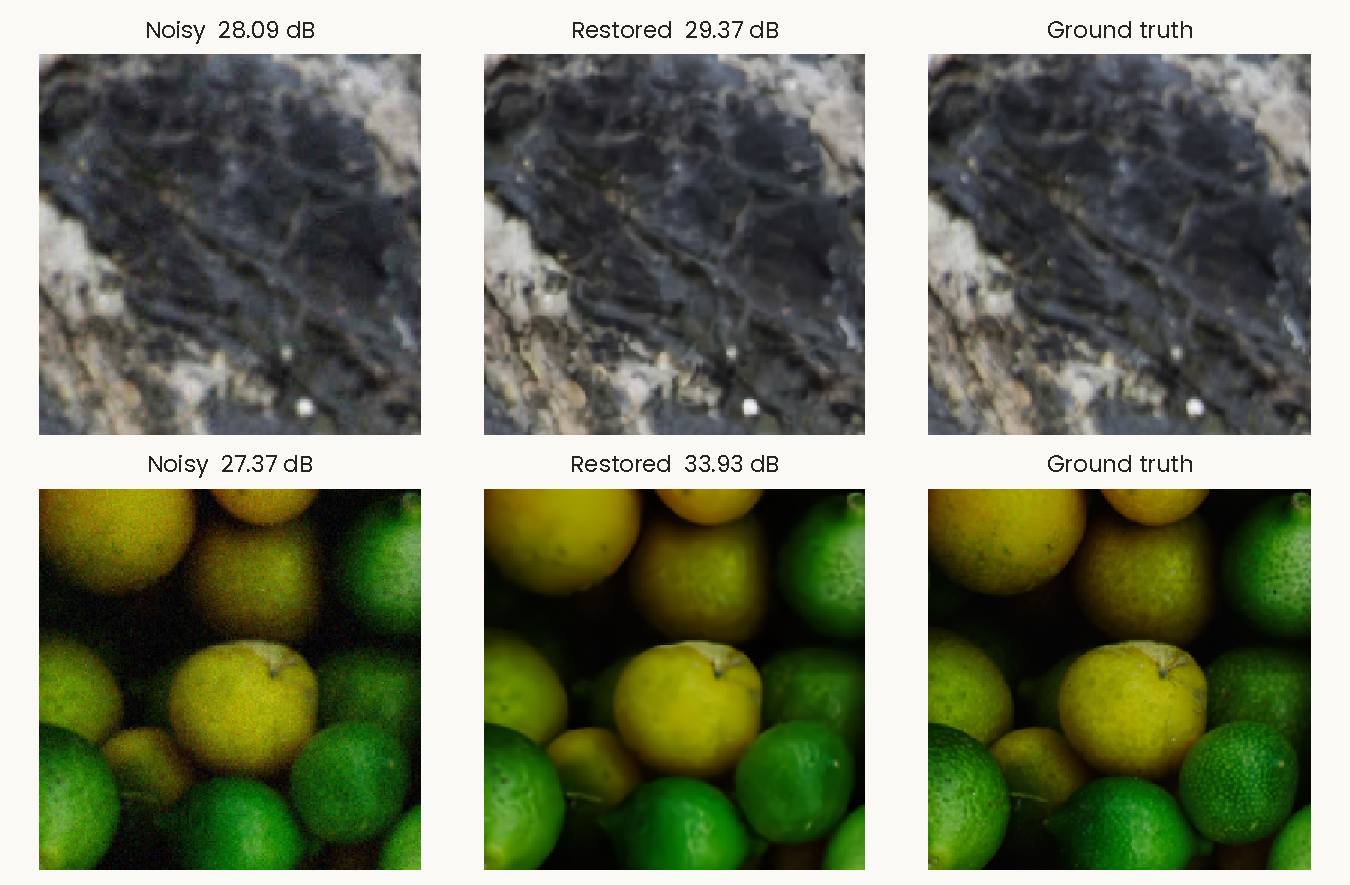
\includegraphics[width=0.92\linewidth]{qualitative_blind.pdf}
		\caption{FFDNet, blind ($\sigma$ map fixed at 27.5/255)}
	\end{subfigure}\\[1ex]
	\begin{subfigure}{\linewidth}
		\centering
		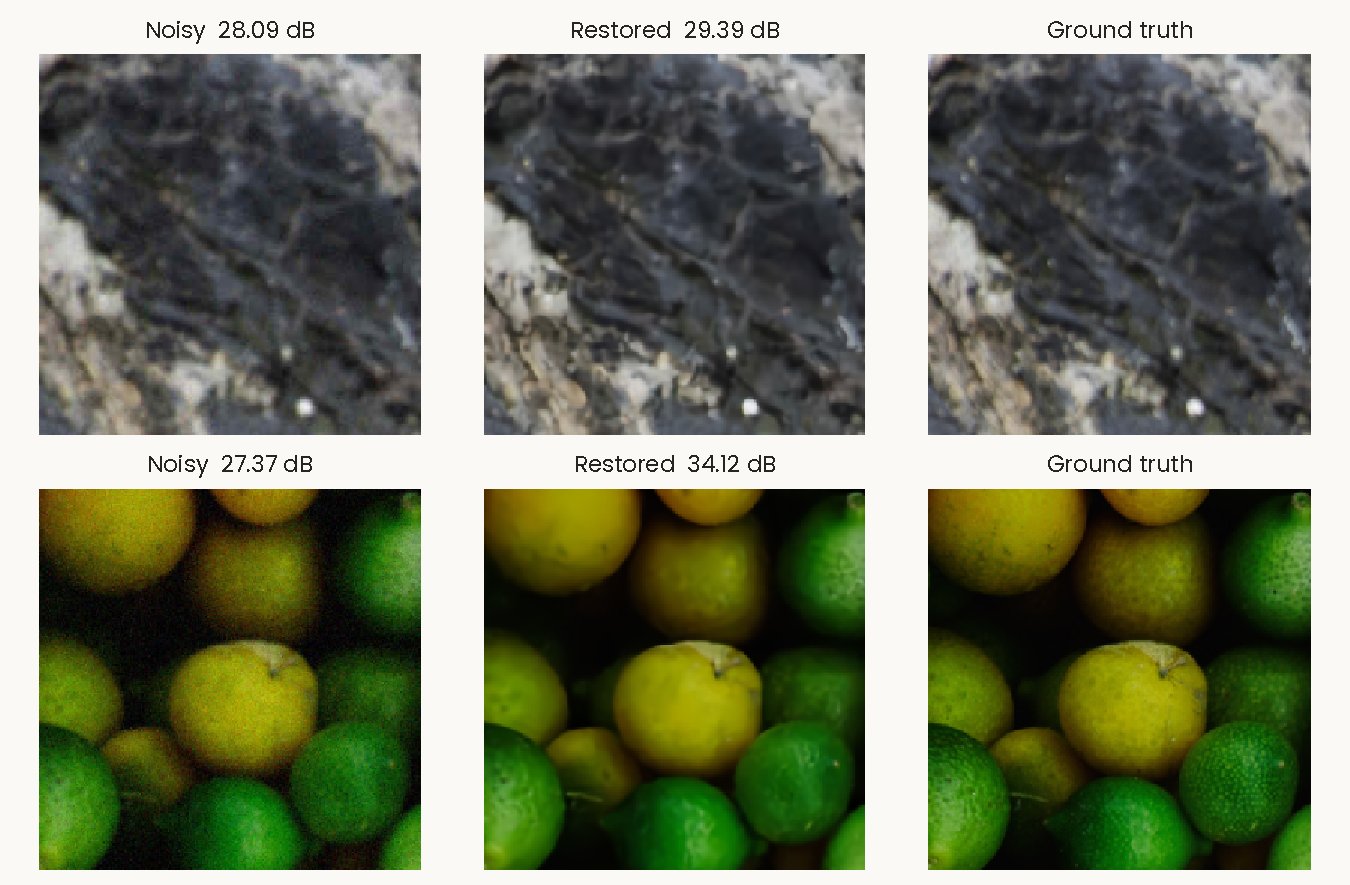
\includegraphics[width=0.92\linewidth]{qualitative_oracle.pdf}
		\caption{FFDNet, oracle (true $\sigma$ map)}
	\end{subfigure}
	\caption{Degraded input, restoration and clean target for the two FFDNet variants.}
	\label{fig:qual-b}
\end{figure}

All four models remove most of the noise and blocking. None of them recovers
the fine texture that blur and downsampling destroyed, which is expected:
those details are not in the input, and a model trained with pixel losses
predicts a smooth average rather than inventing texture. Differences between
models at this scale are subtle, and the saved panels do not include
difference images, so we rely on the quantitative results above rather than
on visual judgement.

\section{Training Convergence}\label{sec:convergence}

Figure~\ref{fig:convergence} plots validation PSNR on the 16 fixed crops
against both updates and wall-clock training time. All four models are close
to a plateau by the end of training. \fcsg{} finishes at 30.59\dB{} on the
crops, below DnCNN (31.66), blind FFDNet (31.97) and oracle FFDNet (32.05),
the same ordering as the full evaluation. Because the curves have flattened,
we have no evidence that simply training \fcsg{} for longer with the same
configuration would close the gap.

\begin{figure}[htbp]
	\centering
	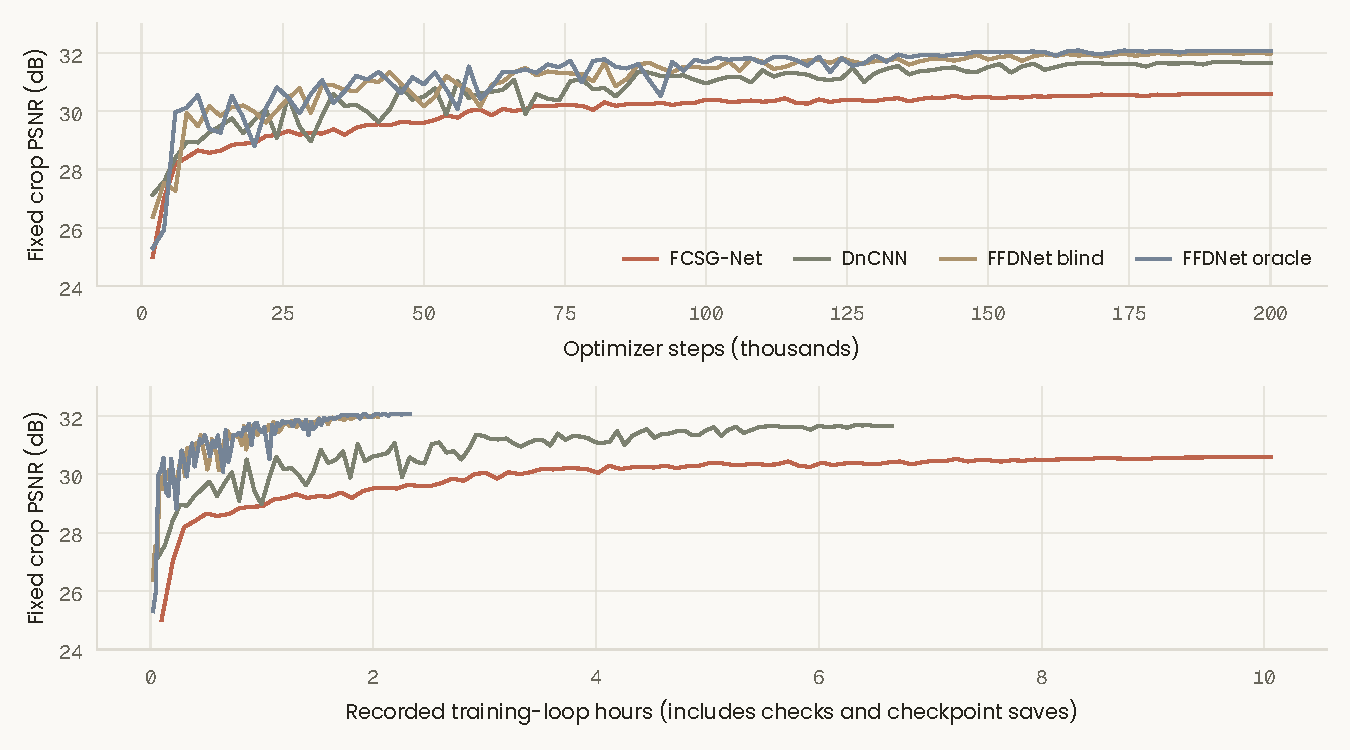
\includegraphics[width=\linewidth]{convergence.pdf}
	\caption{Validation PSNR on 16 fixed crops against updates and training
	time. Crop PSNR is not comparable with the full-image results.}
	\label{fig:convergence}
\end{figure}

The wall-clock panel exposes a cost that the update count hides. \fcsg{}
needed 10.06 hours for 200,000 updates, against 6.66 for DnCNN and about two
for FFDNet. A separate throughput test, excluding warm-up, validation and
checkpointing, measured 5.84 steps per second for \fcsg{}, 9.41 for DnCNN
and 26.67 for FFDNet. Matching the number of updates therefore did not match
the GPU time, and \fcsg{} received the most of it.

\section{Latency, Memory and Tiling}\label{sec:latency}

\paragraph{Latency.} The motivation for a small model is that it should be
cheap to run. Table~\ref{tab:latency} shows that, on the GPU we used, this
did not hold. Measurements are median wall-clock times for one FP32 forward
pass at batch size 1 on a Tesla T4, with TF32 disabled, after 20 warm-up
passes and over 50 timed repetitions.

\begin{table}[htbp]
	\centering
	\caption{Median forward latency (ms) by input size and peak inference memory at $256\times256$ (Tesla T4, FP32, batch 1).}
	\label{tab:latency}
	\begin{tabular}{@{}lrrrr@{}}
		\toprule
		Method & $128^2$ & $256^2$ & $512^2$ & Peak MB at $256^2$ \\
		\midrule
		\fcsg{}          & 5.10 & 19.40 & 75.59 & 51.3 \\
		DnCNN            & 4.22 & 18.04 & 72.47 & 37.8 \\
		FFDNet, blind    & 1.69 &  6.30 & 24.12 & 20.2 \\
		FFDNet, oracle   & 1.69 &  6.35 & 24.62 & 20.2 \\
		\bottomrule
	\end{tabular}
\end{table}

\fcsg{} is the slowest model at every size, slightly behind DnCNN and three
times slower than FFDNet, despite needing an eighth of DnCNN's reported FLOPs
and a third of FFDNet's. It also uses the most memory. We did not profile
individual operators, so the following explanation is our best reading of the
architecture rather than a measurement. Each forward pass runs nine expert
passes, all of them in full, because zero-weighted experts are not skipped.
Depthwise convolutions perform very little arithmetic per byte they read, so
on a GPU their running time is governed by memory traffic, not by the FLOP
count. The network is also made of many small layers, so kernel launch
overhead is a large fraction of the total, and the FFT and inverse FFT add
work that the FLOP estimate counts only approximately. FFDNet, by contrast,
runs one stack of dense $3\times3$ convolutions at half resolution, which is
exactly the kind of workload GPUs are built for.

The practical lesson is that the FLOP budget we set at the start of the
project was the wrong proxy for speed on this hardware. Figure~\ref{fig:cost}
plots quality against both measures. Against FLOPs, \fcsg{} sits far to the
left of the other models. Against latency it sits to the right of FFDNet with
lower quality, so on a T4 it is dominated. Whether the picture changes on a
CPU or a mobile accelerator, where depthwise convolutions are better suited,
remains to be tested.

\begin{figure}[htbp]
	\centering
	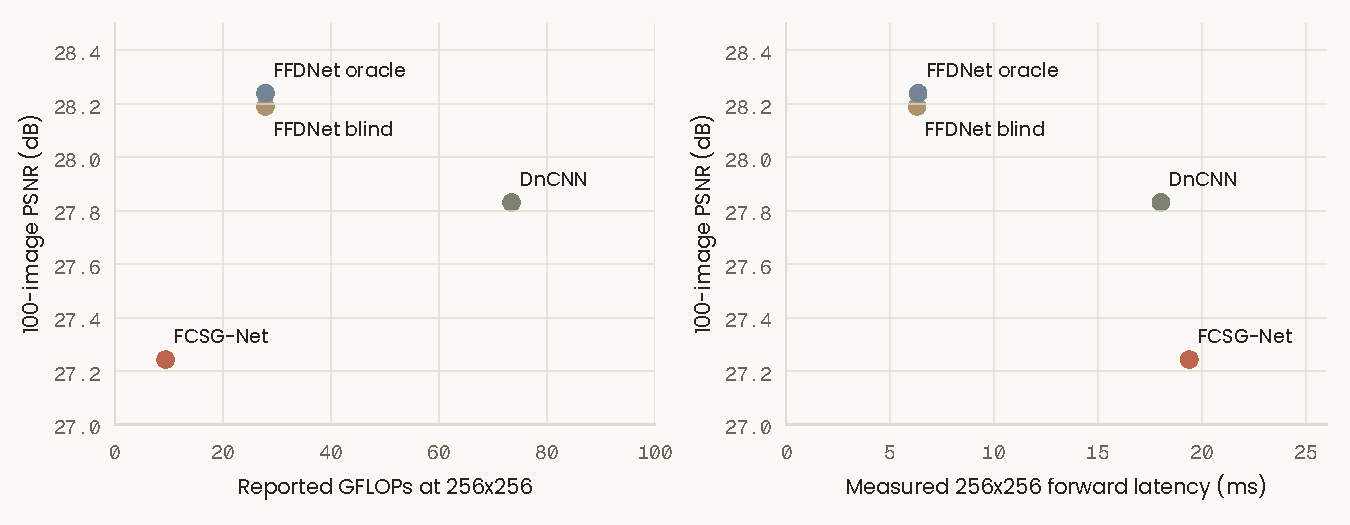
\includegraphics[width=\linewidth]{compute_latency.pdf}
	\caption{Validation PSNR against reported GFLOPs (left) and measured
	$256\times256$ forward latency (right).}
	\label{fig:cost}
\end{figure}

\paragraph{Tiling.} Tiled inference changes what each model sees: the FFT,
the gate's pooling windows and the global pooling in the fusion block all
operate on a $256\times256$ tile rather than the whole image. To measure the
effect we evaluated ten fixed validation images (0801, 0812, \dots, 0900)
with tile sizes of 128, 256 and 512 pixels and a fixed 32-pixel overlap
(Table~\ref{tab:tiling}).

\begin{table}[htbp]
	\centering
	\caption{Mean PSNR (dB) on ten validation images for three tile sizes, 32-pixel overlap.}
	\label{tab:tiling}
	\begin{tabular}{@{}lrrr@{}}
		\toprule
		Method & Tile 128 & Tile 256 & Tile 512 \\
		\midrule
		\fcsg{}         & 26.622 & 26.659 & 26.672 \\
		DnCNN           & 27.330 & 27.341 & 27.343 \\
		FFDNet, blind   & 27.696 & 27.714 & 27.721 \\
		FFDNet, oracle  & 27.730 & 27.748 & 27.756 \\
		\bottomrule
	\end{tabular}
\end{table}

\fcsg{} is the most sensitive to tile size, as expected for a model with
global operations, but the effect is small: going from 256 to 512 pixel
tiles gains 0.013\dB{}, against 0.002\dB{} for DnCNN and about 0.008\dB{}
for FFDNet. This is two orders of magnitude smaller than the 0.6 to 1.0\dB{}
gap in Table~\ref{tab:main}, so tiling does not explain the deficit. The
ten-image means are lower than the 100-image means because the subset
happens to contain harder images; they should be compared only with each
other. Figure~\ref{fig:tiling} shows the paired differences.

\begin{figure}[htbp]
	\centering
	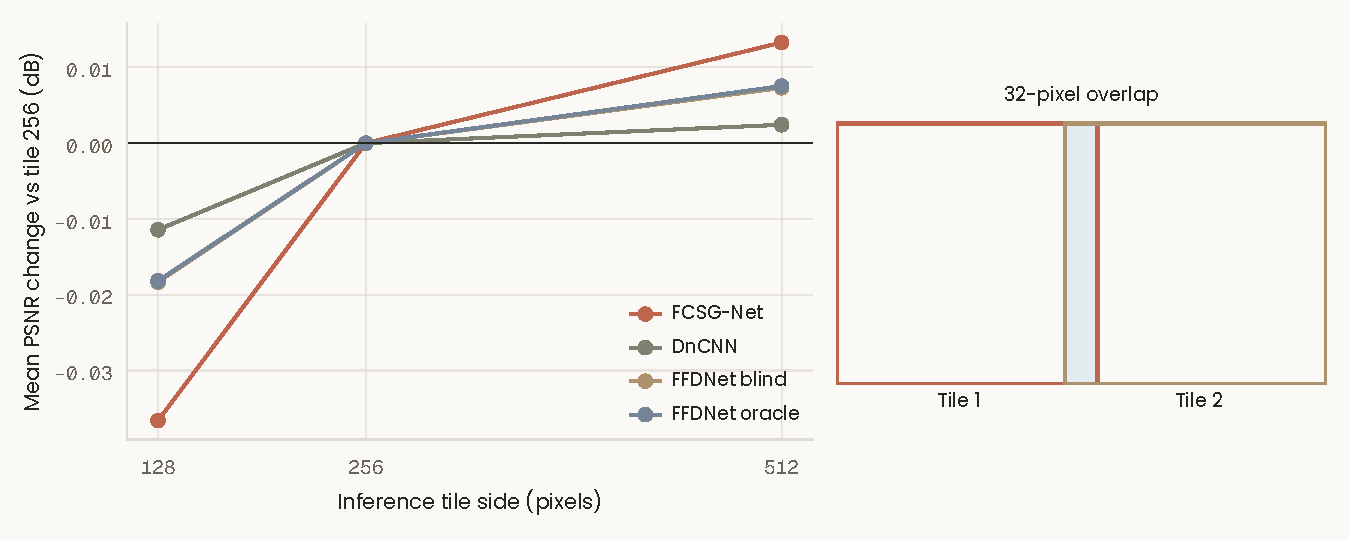
\includegraphics[width=\linewidth]{tiling.pdf}
	\caption{Tile-size sensitivity: PSNR change relative to 256-pixel tiles, and
	the tile and overlap geometry.}
	\label{fig:tiling}
\end{figure}

\thispagestyle{empty}\cleardoublepage

\chapter{Routing Analysis and Ablation}\label{ch:routing}
% LENGTH: 7-9 pages. This is where the project's real contribution lives.
% SOURCES: results/diagnostics/{summary,routing}.json, interventions.csv,
% results/phase4/jobs.json, fcsg-report-assets/live_*.
% RULES:
%  - Correlation is not specialisation. 36 exploratory correlations, 10 source
%    images, no multiple-comparison correction. Say that next to the numbers.
%  - Inference interventions are NOT ablations. Keep them in separate sections.

\section{Spatial Routing Statistics}\label{sec:routing-stats}
% routing_summary.pdf (80 samples = 10 images x 8 seeds).
% High band picks the 3x3 expert almost always (0.999845) yet 7x7 and 5x5 still
% carry ~0.256 and ~0.223 mean weight there.
\begin{figure}[htbp]
	\centering
	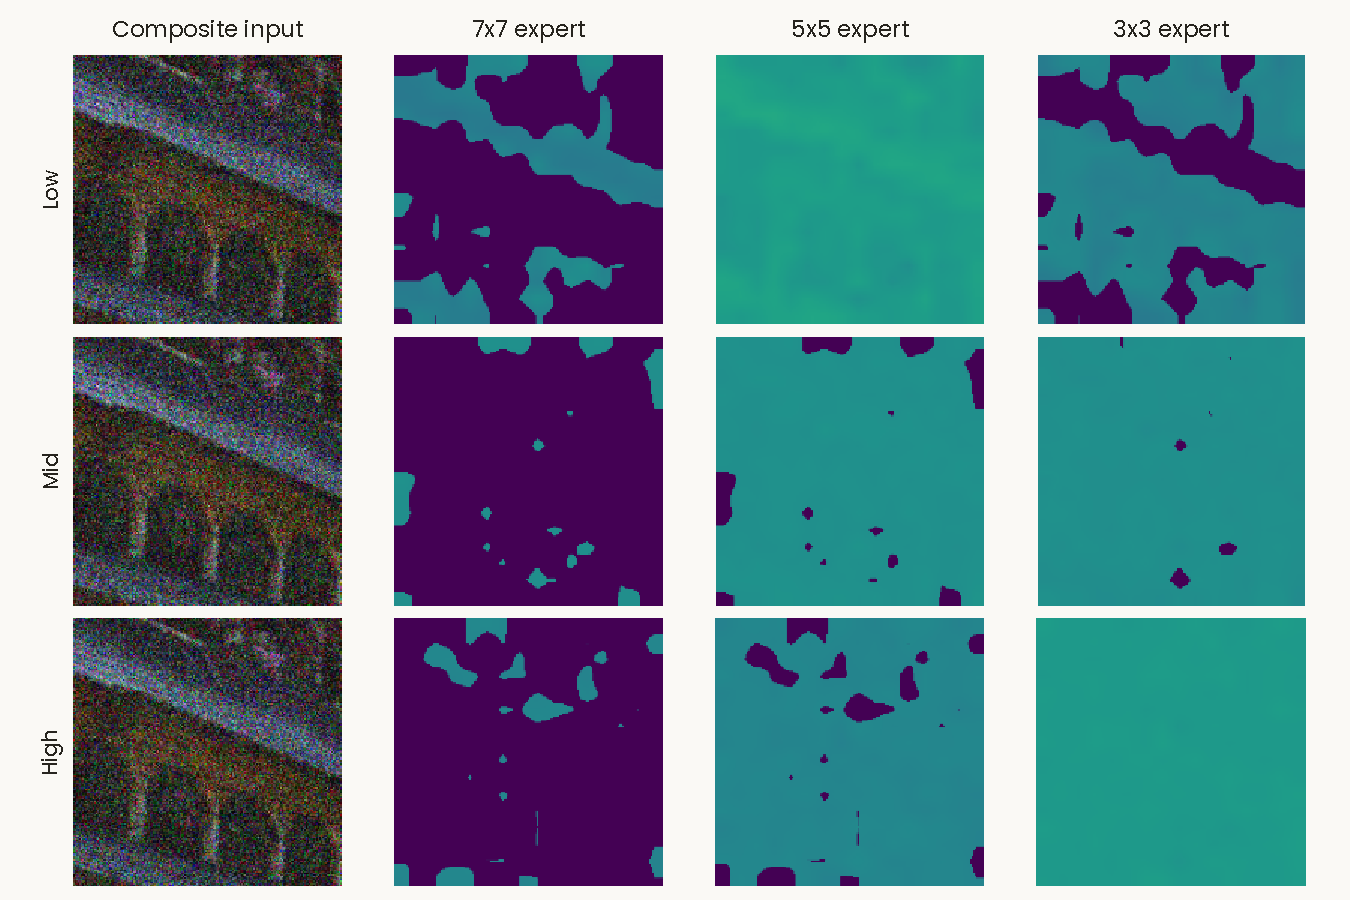
\includegraphics[width=\linewidth]{routing_0834.pdf}
	\caption{Per-band expert weights for DIV2K image 0834. Rows: low, mid, high band.}
	\label{fig:routing-map}
\end{figure}
\todo{write}

\section{Routing Versus Degradation Parameters}\label{sec:routing-corr}
% Within-image-centred Pearson r: high-band 3x3 vs noise sigma +0.809;
% low-band 5x5 +0.798; low-band 7x7 -0.728. Figure correlations_interventions.pdf.
\todo{write, with the caveats above}

\section{Inference-Time Interventions}\label{sec:interventions}
\begin{table}[htbp]
	\centering
	\caption{PSNR change when the trained gate is overridden at inference (10 images).}
	\label{tab:interventions}
	\evidence{results/diagnostics/interventions.csv}
	\begin{tabular}{@{}lrr@{}}
		\toprule
		Intervention & Mean $\Delta$PSNR & Min / Max \\
		\midrule
		Equal weights on selected pair    & $-0.040$\dB & $-0.137$ / $+0.028$ \\
		Uniform weights over all experts  & $-0.372$\dB & $-0.986$ / $+0.163$ \\
		\bottomrule
	\end{tabular}
\end{table}
% Reading: the model depends on WHICH pair it picks far more than on the
% exact mixing weights. That is a useful, specific finding.
\todo{write}

\section{Trained Routing Ablation}\label{sec:ablation}
% fcsg_reference vs fcsg_uniform, seed 1234, 100k steps, matched init.
% STATUS CHECK BEFORE WRITING: results/phase4/jobs.json was last updated
% 2026-10-01 with both runs RUNNING. Pull the finished Kaggle outputs, run the
% 100-image eval, and fill this table. If the runs did not finish, report the
% interim crop numbers as interim and move the conclusion to future work.
\begin{table}[htbp]
	\centering
	\caption{Learned top-2 routing against fixed uniform mixing, matched training.}
	\label{tab:ablation}
	\begin{tabular}{@{}lrrrr@{}}
		\toprule
		Variant & PSNR & SSIM & LPIPS & Trainable params \\
		\midrule
		Reference (learned top-2) & \todo{} & \todo{} & \todo{} & 97,088 \\
		Uniform ($w=1/3$)         & \todo{} & \todo{} & \todo{} & 96,407 \\
		\bottomrule
	\end{tabular}
\end{table}
% Note the ablation removes routing AND entropy regularisation together.
\todo{write once numbers exist}

\section{Discussion}\label{sec:discussion}
% Pull Ch 5 and Ch 6 together: what did routing buy, what did it cost?
% The interventions say the gate matters to THIS checkpoint; only the
% ablation says whether learning a gate beats not having one.
\todo{write}

\thispagestyle{empty}\cleardoublepage

\chapter{Conclusion and Future Work}\label{ch:conclusion}

\section{Summary of Findings}\label{sec:summary}

We set out to test whether a very small restoration network could split an
image into frequency bands and route each band, pixel by pixel, to
convolutional experts of different kernel sizes, and whether the learned
routing would be meaningful. We return to the four objectives of
Section~\ref{sec:objectives}.

\paragraph{O1, build and verify.} \fcsg{} has 97,088 parameters and costs
9.39 reported GFLOPs at $256\times256$, well inside the limits of five million
and ten. It passed every verification check before training: exact band
reconstruction, consistent frequency units across image sizes, gradient flow,
mixed-precision execution, single-image overfitting and exact checkpoint
restoration (Section~\ref{sec:verification}).

\paragraph{O2, trustworthy baselines.} Our FFDNet implementation reproduces
the published CBSD68 result to within 0.01\dB{} using the author's weights,
and our DnCNN training loop reaches 32.65\dB{} on DIV2K for Gaussian
denoising (Section~\ref{sec:baseline-repro}).

\paragraph{O3, matched comparison.} Under one composite degradation and one
training protocol, \fcsg{} reaches 27.24\dB{} PSNR, 0.753 SSIM and 0.396
LPIPS on 100 DIV2K validation images. This is 0.59\dB{} below DnCNN and
0.95\dB{} below blind FFDNet, and it loses to FFDNet on every one of the 100
images. It does so with 82.6\% fewer parameters than DnCNN and 88.6\% fewer
than FFDNet. Its low FLOP count, however, did not make it fast: on a Tesla T4
it is the slowest of the four models (Chapter~\ref{ch:results}).

\paragraph{O4, the routing.} The learned gate varies across the image,
selects the $3\times3$ expert almost everywhere in the high band, and shifts
its weights with the noise level, with within-image correlations up to
$r=+0.81$. Overriding its selections at inference costs 0.37\dB{} on average,
while flattening its weights within the selected pair costs only 0.04\dB{},
so the trained model depends on which experts are chosen more than on how
they are mixed (Chapter~\ref{ch:routing}).

In short, frequency-band routing produced a small model whose behaviour can
be inspected and related to the degradation, but within our budget it did
not produce a model that is better or faster than simple convolutional
baselines.

\section{Limitations}\label{sec:limitations}

Several limitations bound how far these results can be taken.

Each model was trained once with an unfixed seed, so we have no estimate of
run-to-run variance. The consistency of the gap across images makes it
unlikely to be an accident of one seed, but small differences, such as
between the two FFDNet variants, cannot be interpreted. All results are on
the DIV2K validation split, which was also used to monitor training; there is
no untouched test set.

The degradation is synthetic. Real archival photographs suffer from fading,
scratches, dust, colour casts and scanner artefacts that our pipeline does
not model, and we did not evaluate on real archival images or ask people to
judge the results. The good performance of any of these models on our data
says nothing yet about real archives.

The routing analysis uses ten source images. Its correlations are
exploratory, the four degradation parameters vary together, and there is no
correction for the number of comparisons. The inference interventions
measure the trained model's dependence on its gate, not the value of having a
gate during training.

The cost measurements cover one GPU, the Tesla T4, at batch size 1 in FP32.
We did not profile individual operators, so our explanation of why \fcsg{} is
slow is a reasoned account rather than a measurement. We did not measure
latency on CPUs or mobile hardware, nor peak training memory at batch 16.

Finally, \fcsg{} computes all nine expert passes regardless of the gate, so
its sparse routing does not save computation.

\section{Future Work}\label{sec:future}

The most important next step is a matched training ablation: train \fcsg{}
and an otherwise identical model with fixed uniform weights from the same
initialisation and seed, and compare them on the full validation set,
preferably with several seeds each. This is the only experiment that can
show whether learning a router helps, rather than whether a trained model
depends on its router. Related ablations would replace the three kernel sizes
with three identical $3\times3$ experts, replace the spatial gate with a
single per-image gate, replace SE fusion with plain concatenation, and
replace the soft masks with hard ones. Each of these isolates one design
decision of Chapter~\ref{ch:method}.

The second direction is to turn sparse weights into sparse computation. Since
the trained model mostly cares about which two experts are chosen, skipping
the third expert in tiles where it is never selected could reduce the
running cost by up to a third. This should be preceded by an operator-level
profile, because if latency is dominated by memory traffic and launch
overhead, removing arithmetic may not help much. Measuring latency on a CPU
and on a mobile accelerator would show whether the model's low FLOP count
is worth more on hardware that suits depthwise convolutions.

Third, the capacity gap could be addressed directly by widening the experts
within the parameter budget, which is about fifty times larger than what the
model uses. The compute budget is nearly exhausted, so this would have to go
together with cheaper expert evaluation, for example by sharing one
unshuffled feature map across bands. Letting the gate see a larger context than a $16\times16$
window may also help.

Finally, any claim about archival restoration needs real archival
photographs, a controlled degradation sweep to separate the effect of each
corruption on the routing, and a held-out test set that was never used
during development.

\thispagestyle{empty}\cleardoublepage

% ---------------------------------------------------------------- back matter
\rhead{\textit{References}}
\lhead{}
\renewcommand\bibname{References}
\bibliographystyle{Ref/IEEEtran}   % CS/EE norm; the template lists it as an option
{
	\fontsize{10}{12}
	\selectfont
	\addcontentsline{toc}{chapter}{References}
	\bibliography{Ref/references}
}
\cleardoublepage

\appendix
\chapter{Reproducibility record}\label{app:repro}

\section{Code and environment}

The project repository at \url{https://github.com/whynotramaa/fcsg-capstone}
holds all code, configuration files, logs and evaluation outputs. Model code
is in \texttt{models/} and \texttt{src/fcsg\_net/}, training in
\texttt{training/train.py}, and evaluation and plotting in
\texttt{evaluation/}. A configuration file in \texttt{configs/} selects each
model. The four composite runs use \texttt{fcsg.toml},
\texttt{dncnn\_composite.toml}, \texttt{ffdnet\_blind.toml} and
\texttt{ffdnet\_composite.toml}. They differ only in the model and the noise
map.

We ran training, verification and diagnostics on Kaggle with an NVIDIA Tesla
T4, Python 3.12.13, PyTorch 2.10.0 with CUDA 12.8, NumPy 2.0.2 and Pillow
11.3.0. Local machines were only for editing and packaging code.

\section{Where each result comes from}

\begin{table}[htbp]
	\centering
	\caption{Source files for the results in this report.}
	\label{tab:sources}
	\small
	\begin{tabular}{@{}ll@{}}
		\toprule
		Result & File \\
		\midrule
		Verification checks (Table~\ref{tab:gates}) & \texttt{results/milestone\_run\_20260925/} \\
		Gaussian DnCNN (Table~\ref{tab:gaussian})   & \texttt{results/benchmark.csv} \\
		Composite results (Table~\ref{tab:main})     & \texttt{results/phase3/*/evaluation.json} \\
		Per-image results (Appendix~\ref{app:per-image}) & \texttt{results/phase3/per\_image\_scores.csv} \\
		Training curves                              & \texttt{results/phase3/*/train\_log.csv} \\
		Latency, tiling, routing                     & \texttt{results/diagnostics/} \\
		Figures                                      & \texttt{output/pdf/fcsg-report-assets/} \\
		\bottomrule
	\end{tabular}
\end{table}

\section{Artefact identifiers}

Each Kaggle run packed its source code into a bundle and recorded the
bundle's SHA-256 hash. Even after later edits, the hash pins down the exact
code behind each result. Table~\ref{tab:hashes} lists the first sixteen hex
digits of each hash. The source manifests hold the full values.

\begin{table}[htbp]
	\centering
	\caption{SHA-256 identifiers (first 16 hex digits) of the evaluated artefacts.}
	\label{tab:hashes}
	\small
	\begin{tabular}{@{}ll@{}}
		\toprule
		Artefact & SHA-256 prefix \\
		\midrule
		Composite training source bundle & \texttt{85d6e16f72ead013} \\
		Diagnostics source bundle        & \texttt{d473bc10b0ad0c1e} \\
		5,000-pair dataset manifest      & \texttt{7ce7f310bdb4d2d5} \\
		\fcsg{} checkpoint               & \texttt{8db0bb0f3c251ddc} \\
		DnCNN checkpoint                 & \texttt{afb0abfa022ede04} \\
		FFDNet blind checkpoint          & \texttt{981560c18cbea134} \\
		FFDNet oracle checkpoint         & \texttt{ef9560e8ed1ebae0} \\
		\bottomrule
	\end{tabular}
\end{table}

\section{How to reproduce}

\begin{enumerate}
	\item Attach the DIV2K dataset to a Kaggle notebook with a GPU. Run
	\texttt{notebooks/checks.ipynb}, then the bundled milestone notebook
	\texttt{notebooks/phase1\_phase2.ipynb}. Both stop at the first failed
	check.
	\item Build and push one training notebook per configuration with
	\texttt{python notebooks/build\_phase3.py fcsg ffdnet\_blind
	ffdnet\_composite dncnn\_composite}. To continue a run that outlasts one
	session, rebuild it with \texttt{--resume}. It picks up from its last
	checkpoint.
	\item At 200,000 updates, each run evaluates the 100 validation images and
	writes \texttt{evaluation.json} and \texttt{status.json}.
	\item To measure latency, tiling and routing, build the diagnostic notebook
	with \texttt{python notebooks/build\_diagnostics.py}. Draw the figures with
	\texttt{python evaluation/plots.py}.
\end{enumerate}

\cleardoublepage
\chapter{Per-Image Results}\label{app:per-image}
% 100 images x 4 methods. Generate this table from
% results/phase3/per_image_scores.csv with a script, never by hand.
% Suggested: thesis/tools/per_image_table.py writes appendix/per_image_rows.tex,
% then \input it inside a longtable here. Columns: image, input PSNR, then
% output PSNR for DnCNN, FFDNet blind, FFDNet oracle, FCSG-Net.
% If page count is tight, drop this appendix; the CSV is in the repo.
\todo{generate table}

\cleardoublepage

% Dissemination: keep only if a paper/poster/preprint exists. Otherwise delete.
%\rhead{\textit{Dissemination}}
%\lhead{}
%\input{Ref/Dissemination}
%\thispagestyle{empty}
%\cleardoublepage

% Index: the template ends with \indexColumns{3}\indexPage. It is only useful
% if someone tags terms with \index{...} while writing. Drop it otherwise.
%\indexColumns{3}
%\indexPage
\end{document}
